%input macros (i.e. write your own macros file called MacroFile1.tex)
\newcommand{\PdfPsText}[2]{
  \ifpdf
     #1
  \else
     #2
  \fi
}

\newcommand{\IncludeGraphicsH}[3]{
  \PdfPsText{\includegraphics[height=#2]{#1}}{\includegraphics[bb = #3, height=#2]{#1}}
}

\newcommand{\IncludeGraphicsW}[3]{
  \PdfPsText{\includegraphics[width=#2]{#1}}{\includegraphics[bb = #3, width=#2]{#1}}
}

\newcommand{\InsertFig}[3]{
  \begin{figure}[!htbp]
    \begin{center}
      \leavevmode
      #1
      \caption{#2}
      \label{#3}
    \end{center}
  \end{figure}
}


%%% Local Variables: 
%%% mode: latex
%%% TeX-master: "~/Documents/LaTeX/CUEDThesisPSnPDF/thesis"
%%% End: 


 \documentclass[twoside,12pt]{Classes/CUEDthesisPSnPDF}


\ifpdf
    \pdfinfo { /Title  (CUED PhD and MPhil Thesis Classes)
               /Creator (TeX)
               /Producer (pdfTeX)
               /Author (Lars Barquist lb14@sanger.ac.uk)
               /CreationDate (D:20030101000000)  %format D:YYYYMMDDhhmmss
               /ModDate (D:20030815213532)
               /Subject (High-throughput Experimental and Computational Studies of Bacterial Evolution)
               /Keywords (PhD, Thesis)}
    \pdfcatalog { /PageMode (/UseOutlines)
                  /OpenAction (fitbh)  }
\fi


\title{High-throughput Experimental and Computational Studies of Bacterial Evolution}

\ifpdf
  \author{Lars Barquist}
  \collegeordept{Queens' College}
  \university{University of Cambridge}
% insert below the file name that contains the crest in-place of 'UnivShield'
  \crest{
\includegraphics[width=29mm]{UnivShield}}
\else
  \author{Lars Barquist}
  \collegeordept{Queens' College}
  \university{University of Cambridge}
% insert below the file name that contains the crest in-place of 'UnivShield'
  \crest{
\includegraphics[bb = 0 0 0 0, width=30mm]{UnivShield}}
\fi
%
% insert below the file name that contains the crest in-place of 'UnivShield'
% \crest{\IncludeGraphicsW{UnivShield}{40mm}{14 14 73 81}}
%
%\renewcommand{\submittedtext}{change the default text here if needed}
\degree{Doctor of Philosophy}
\degreedate{XX August 2013}

% turn of those nasty overfull and underfull hboxes
\hbadness=10000
\hfuzz=50pt
\usepackage{lscape}
% Put all the style files you want in the directory StyleFiles and usepackage like this:
\usepackage{StyleFiles/watermark}
\usepackage[font=small,labelfont=bf]{caption}
\usepackage{url}
\usepackage{textcomp}
\usepackage{lscape}
\usepackage{siunitx}
\usepackage{booktabs}
\usepackage{longtable}
\usepackage{multirow}
\usepackage[table]{xcolor}
\usepackage{nomencl}
\usepackage{array}

%sort out the headers
\usepackage{fancyhdr}
\usepackage{rotating}
\usepackage{flexisym}
%nice formatting
\usepackage{microtype}
\fancyhf{}
\fancyfoot{}

%Switch to biblatex
\usepackage{babel}% Recommended
\usepackage{csquotes}
\addbibresource{References/references.bib}

\raggedbottom

\DefineBibliographyStrings{english}{%
  in = {},
}

% Comment out the next line to get single spacing
\onehalfspacing


\begin{document}
\maketitle

%set the number of sectioning levels that get number and appear in the contents
\setcounter{secnumdepth}{3}
\setcounter{tocdepth}{3}

\thispagestyle{empty}
\newpage

\frontmatter % book mode only
\pagenumbering{roman}
%% Thesis Dedictation ---------------------------------------------------


%\begin{dedication} %this creates the heading for the dedication page
\vspace*{\fill}
\begingroup
\center{\textit{Arrakis teaches the attitude of the knife -- chopping off what's incomplete and saying: ``Now it's complete because it's ended here.''}}

 \hfill Collected Sayings of Muad'dib

\endgroup
\vspace*{\fill}


%\end{dedication}

% ----------------------------------------------------------------------

%%% Local Variables: 
%%% mode: latex
%%% TeX-master: "../thesis"
%%% End: 

%\thispagestyle{empty}
\cleardoublepage
\thispagestyle{empty}
% \pagebreak[4]
% \hspace*{1cm}
% \pagebreak[4]
% \hspace*{1cm}
% \pagebreak[4]
%\usepackage[round,colon,authoryear]{natbib}

\chapter{Declaration}
%\ifpdf
%    \graphicspath{{Chapter0/Chapter0Figs/PNG/}{Chapter0/Chapter0Figs/PDF/}{Chapter0/Chapter0Figs/}}
%\else
%    \graphicspath{{Chapter0/Chapter0Figs/EPS/}{Chapter0/Chapter0Figs/}}
%\fi

%\begin{document}
\begin{center}
	\textsc{High-throughput Experimental and Computational Studies of Bacterial Evolution}
\end{center}
%\newline{}

The work presented in this dissertation was carried out at the Wellcome Trust Sanger Institute between October 2009 and August 2013. This dissertation is the result of my own work and includes nothing which is the outcome of work done in collaboration except where specifically indicated in the text. This thesis does not exceed the limit of 60,000 words as specified by the Faculty of Biology Degree Committee. This thesis has been typeset in 12pt Computer Modern font using \LaTeX{} according to the specifications set by the Board of Graduate Studies and the Faculty of Biology Degree Committee.
%\end{document}
% ------------------------------------------------------------------------


%%% Local Variables: 
%%% mode: latex
%%% TeX-master: "../thesis"
%%% End: 

\thispagestyle{empty}
\cleardoublepage

%% Thesis Acknowledgements ------------------------------------------------


\begin{acknowledgementslong} 
%uncommenting this line, gives a different acknowledgements heading
%\begin{acknowledgements}      %this creates the heading for the acknowlegments




%\end{acknowledgements}
\end{acknowledgementslong}

% ------------------------------------------------------------------------

%%% Local Variables: 
%%% mode: latex
%%% TeX-master: "../thesis"
%%% End: 

%
% Thesis Abstract -----------------------------------------------------


%\begin{abstractslong}    %uncommenting this line, gives a different abstract heading
\begin{abstracts}        %this creates the heading for the abstract page

The work in this thesis is concerned with the study of bacterial adaptation on short and long timescales. In the first section, consisting of three chapters, I describe a recently developed high-throughput technology for probing gene function, transposon-insertion sequencing, and its application to the study of functional differences between two important human pathogens, \textit{Salmonella enterica} subspecies \textit{enterica} serovars Typhi and Typhimurium. In a first study, I use transposon-insertion sequencing to probe differences in gene requirements during growth on rich laboratory media, revealing differences in serovar requirements for genes involved in iron-utilization and cell-surface structure biogenesis, as well as in requirements for non-coding RNA. In a second study I more directly probe the genomic features responsible for differences in serovar pathogenicity by analyzing transposon-insertion sequencing data produced following a two hour infection of human macrophage, revealing large differences in the selective pressures felt by these two closely related serovars in the same environment.

The second section, consisting of two chapters, uses statistical models of sequence variation, i.e. covariance models, to examine the evolution of intrinsic termination across the bacterial kingdom. A first collaborative study provides background and motivation in the form of a method for identifying Rho-independent terminators using covariance models built from deep alignments of experimentally-verified terminators from \textit{Escherichia coli} and \textit{Bacillus subtilis}. In the course of the development of this method I discovered a novel putative intrinsic terminator in \textit{Mycobacterium tuberculosis}. In the final chapter, I extend this approach to de novo discovery of intrinsic termination motifs across the bacterial phylogeny. I present evidence for lineage-specific variations in canonical Rho-independent terminator composition, as well as discover seven non-canonical putative termination motifs. Using a collection of publicly available RNA-seq datasets, I provide evidence for the function of some of these elements as bona fide transcriptional attenuators.

\end{abstracts}
%\end{abstractlongs}


% ----------------------------------------------------------------------


%%% Local Variables: 
%%% mode: latex
%%% TeX-master: "../thesis"
%%% End: 

%\include{References/references}

\tableofcontents
\listoffigures
\listoftables
\makenomenclature
\renewcommand{\nomname}{List of Symbols}
\printnomenclature[10em]
\addcontentsline{toc}{chapter}{List of Symbols}

\nomenclature{A, C, G, T, U}{Adenine, Cytosine, Guanine, Thymine, Uracil}
\nomenclature[R]{Ala, A}{Alanine}
\nomenclature[R]{Arg, R}{Arginine}
\nomenclature[R]{Asn, N}{Asparagine}
\nomenclature[R]{Asp, D}{Aspartic acid (Aspartate)}
\nomenclature[R]{Cys, C}{Cystine}
\nomenclature[R]{Gln, Q}{Glutamine}
\nomenclature[R]{Glu, E}{Glutamic acid (Glutamate)}
\nomenclature[R]{Gly, G}{Glycine}
\nomenclature[R]{His, H}{Histidine}
\nomenclature[R]{Ile, I}{Isoleucine}
\nomenclature[R]{Leu, L}{Leucine}
\nomenclature[R]{Lys, K}{Lysine}
\nomenclature[R]{Met, M}{Methionine}
\nomenclature[R]{Phe, F}{Phenylalanine}
\nomenclature[R]{Pro, P}{Proline}
\nomenclature[R]{Ser, S}{Serine}
\nomenclature[R]{Thr, T}{Threonine}
\nomenclature[R]{Trp, W}{Tryptophan}
\nomenclature[R]{Tyr, Y}{Tyrosine}
\nomenclature[R]{Val, V}{Valine}



\mainmatter % book mode only
\fancyhead[LO,RE]{\slshape Chapter \nouppercase \leftmark}
\fancyfoot[C]{\thepage}



%%%% Thesis Introduction --------------------------------------------------
\chapter{Introduction}
\markboth{Introduction}{Introduction}
\ifpdf
    \graphicspath{{Introduction/IntroductionFigs/PNG/}{Introduction/IntroductionFigs/PDF/}{Introduction/IntroductionFigs/}}
\else
    \graphicspath{{Introduction/IntroductionFigs/EPS/}{Introduction/IntroductionFigs/}}
\fi

Bacteria possess a remarkable ability to adapt. This ability has allowed bacteria colonize almost every environ on Earth, from deep sea hydrothermal vents \parencite{Jorgensen1992} to cryogenic brine lakes \parencite{Murray2012} to animal hosts \parencite{Finlay1997}. Indeed, the ability of bacteria to establish symbiotic relationships with host cells was a critical step in the origin of so-called ``higher" eukaryotic life \parencite{Sagan1967}. While the origins of some adaptations, such as the differing bauplans 

Several factors likely contribute to this ability, including large population sizes, wide-spread homologous recombination, and a capacity for horizontal gene transfer. These factors, particularly homologous recombination, 
%\usepackage[round,colon,authoryear]{natbib}

\chapter{Querying bacterial genomes with transposon-insertion sequencing}
\label{sec:chapter_piRNAs}
\ifpdf
    \graphicspath{{Chapter1/Chapter1Figs/PNG/}{Chapter1Chapter1Figs/PDF/}{Chapter1/Chapter1Figs/}}
\else
    \graphicspath{{Chapter1/Chapter1Figs/EPS/}{Chapter1/Chapter1Figs/}}
\fi


\textit{This chapter is an expansion of the previously published article ``Approaches to querying bacterial genomes using transposon-insertion sequencing'' \parencite{Barquist2013}. Amy K. Cain and Christine J. Boinett (Pathogen Genomics, Wellcome Trust Sanger Institute) contributed to the research of the original article. All final language is my own.}

\section{Introduction}

A common approach to identifying genomic regions involved in survival under a particular set of conditions is to screen large pools of mutants simultaneously. This can be done with defined mutants \parencite{Baba2006, Hobbs2010}; however, the construction of defined mutant libraries is labor-intensive and requires accurate genomic annotation, which can be particularly difficult to define for non-coding regions. An alternative to defined libraries is the construction and analysis of random transposon-insertion libraries. The original application of this method used DNA\nomenclature{DNA}{Deoxyribonucleic acid} hybridization to track uniquely tagged transposon-insertions in {\it Salmonella enterica} serovar Typhimurium over the course of BALB/c\nomenclature{BALB}{Bagg albino} mouse infection \parencite{Hensel1995}. DNA hybridization was eventually superseded by methods that used microarray detection of the genomic DNA flanking insertion sites, variously known as TraSH\nomenclature{TraSH}{Transposon site hybridization}, MATT\nomenclature{MATT}{Microarray tracking of transposon mutants}, and DeADMAn\nomenclature{DeADMAn}{Designer microarrays for defined mutant analysis} (reviewed in \cite{Mazurkiewicz2006}). However, these methods suffered from many of the problems microarrays generally suffer from: difficulty detecting low-abundance transcripts, mis-hybridization, probe saturation, and difficulty identifying insertion sites precisely.

The application of high-throughput sequencing to the challenge of determining insertion location and prevalence solves many of these problems. Interestingly, the first application of transposon-insertion sequencing, developed by \textcite{Hutchison1999}, actually predates the development of microarray-based methods. However, this was applied to libraries of only approximately 1000 transposon mutants in highly reduced {\it Mycoplasma} genomes, and the difficulty of sequencing at the time prevented wide spread adoption or high resolution. Modern high-throughput sequencing technology allows the methods discussed in this review to routinely monitor as many as one million mutants simultaneously in virtually any genetically tractable microorganism. 

\section{Protocols}
Several methods were developed concurrently for high-throughput sequencing of transposon-insertion sites: TraDIS\nomenclature{TraDIS}{Transposon directed insertion sequencing} \parencite{Langridge2009a}, INSeq\nomenclature{INSeq}{Insertion sequencing} \parencite{Goodman2009}, HITS\nomenclature{HITS}{High-throughput insertion tracking by deep sequencing} \parencite{Gawronski2009}, and Tn-seq \nomenclature{Tn-seq}{Transposon mutagenesis and sequencing}\parencite{Opijnen2009} followed by Tn-seq Circle \parencite{Gallagher2011} and refinements to the INSeq protocol \parencite{Goodman2011}. All of these protocols follow the same basic workflow with minor variations (see Figure \ref{fig:protocols}; Table \ref{tab:studies}): transposon mutagenesis and construction of pools of single insertion mutants; enrichment of transposon-insertion junctions; and finally, in some protocols a purification step either precedes or follows PCR\nomenclature{PCR}{Polymerase chain reaction} enrichment before sequencing.

\begin{figure}[h]
\begin{center}
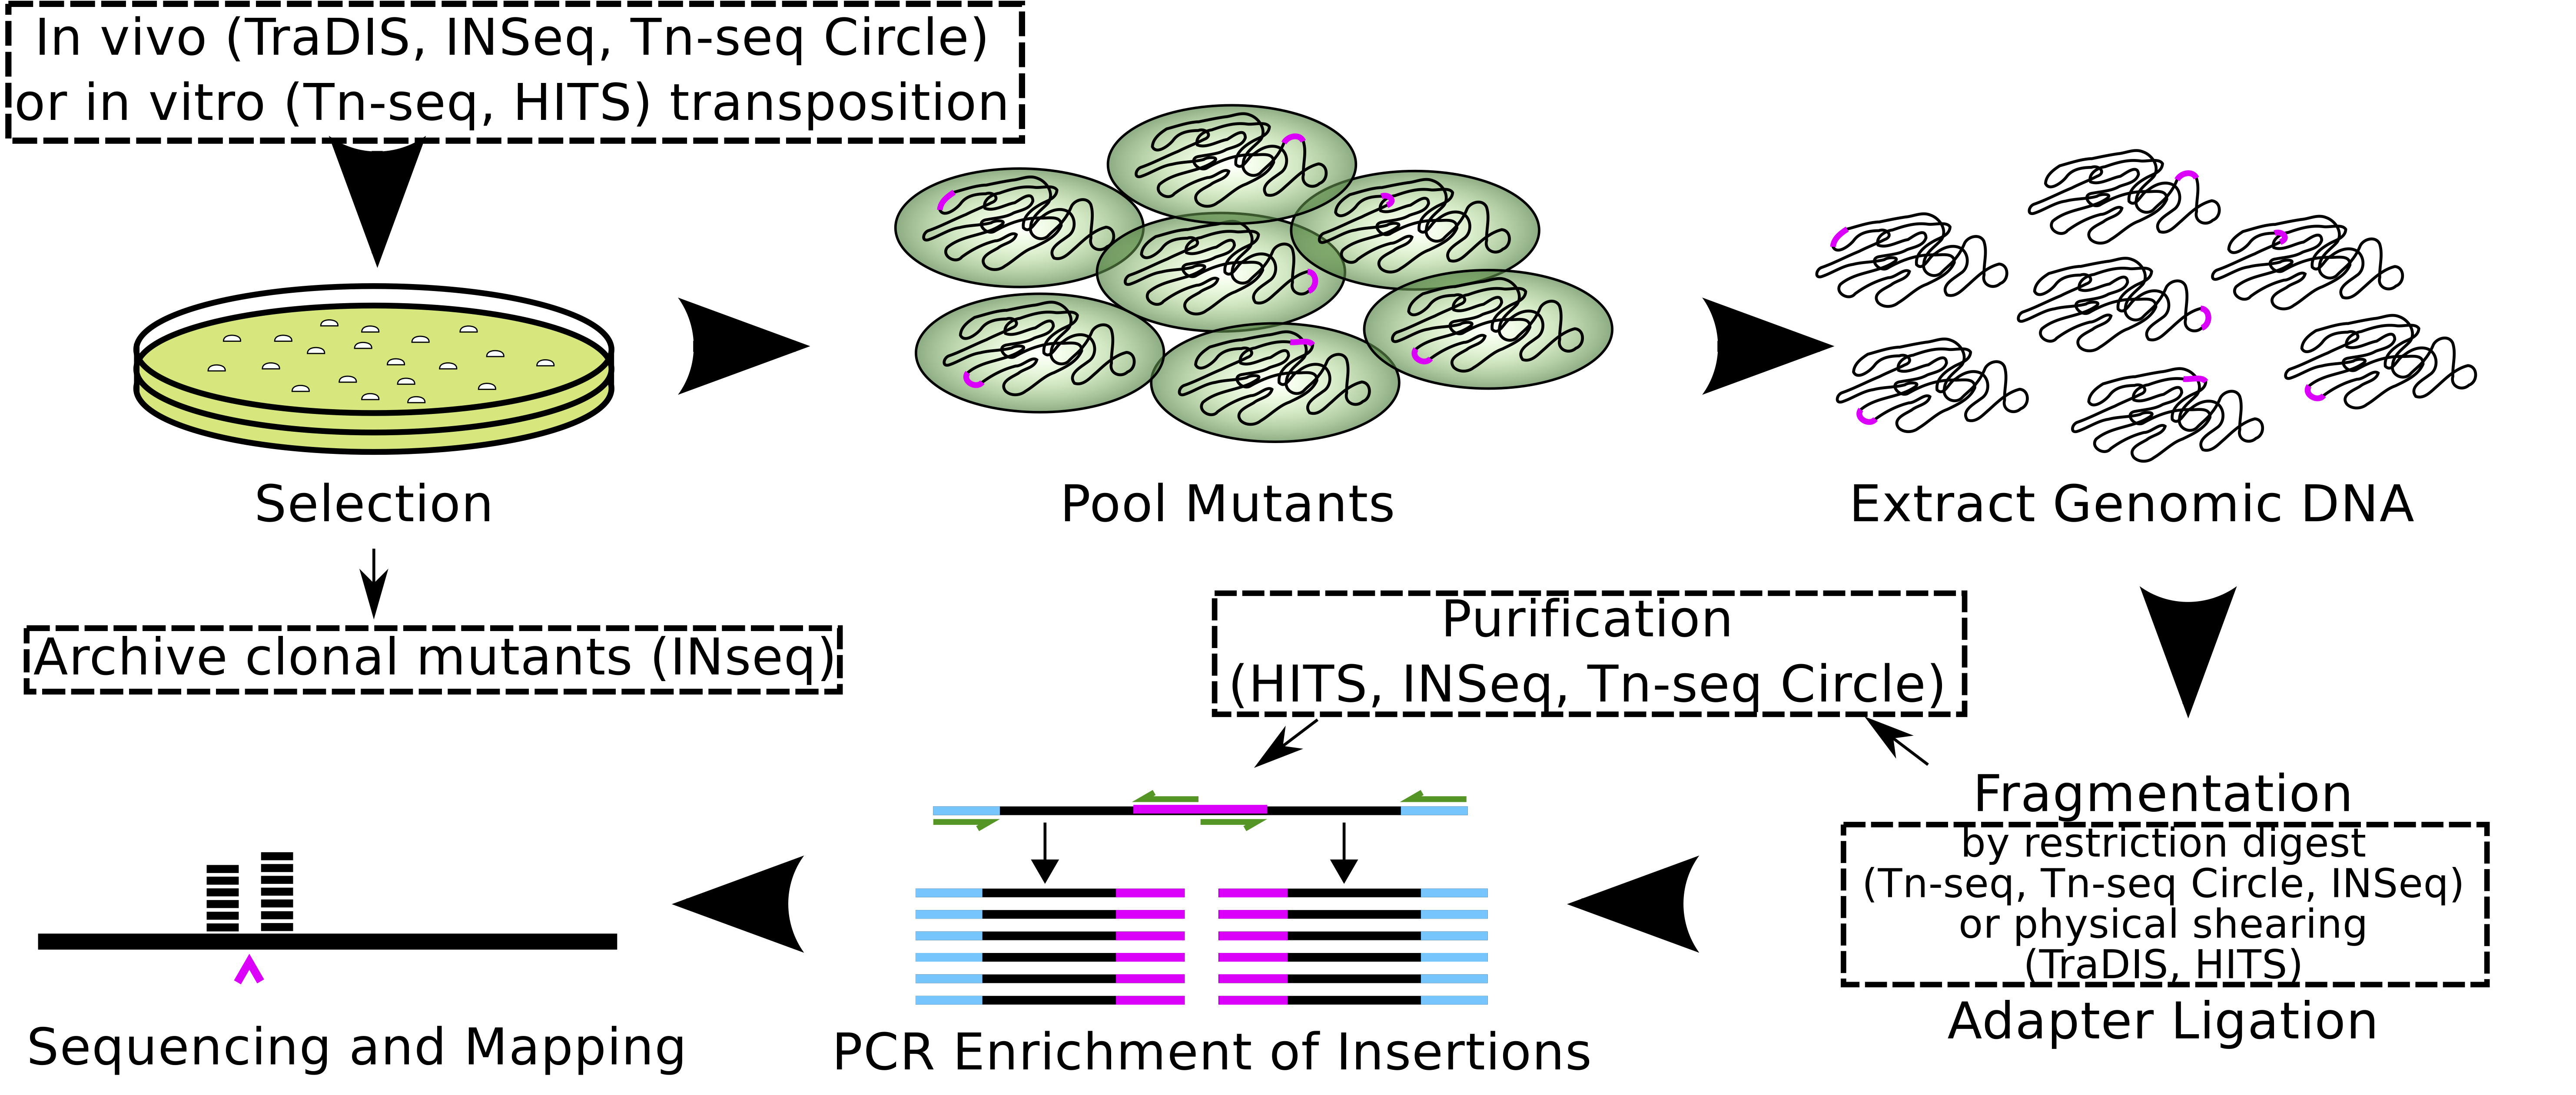
\includegraphics[width=14cm]{protocols}
\caption[Transposon-insertion sequencing protocols]{\textbf{Transposon-insertion sequencing protocols.} An illustration of the workflow typical of transposon-insertion sequencing protocols. Transposons are represented by pink lines, sequencing adaptors by blue, genomic DNA by black, and PCR primers by green. Mutants are generated through either in vivo or in vitro transposition and subsequent selection for antibiotic resistance. These mutants are pooled, and optionally competed in test conditions, then genomic DNA is extracted and fragmented by restriction digest or physical shearing. Sequencing adaptors are ligated, some protocols then perform a step to purify fragments containing transposon insertions, and PCR with transposon- and adapter-specific primers is used to specifically enrich for transposon-containing fragments. The fragments are then sequenced and mapped back to a reference genome to uniquely identify insertion sites with nucleotide-resolution. Dashed boxes indicate steps which differ between protocols.
} 
 \label{fig:protocols}
\end{center}
\end{figure}

\subsection{Transposon mutagenesis}
Most studies have used either Tn{\it 5} or Mariner transposon derivatives. Tn{\it 5} originated as a bacterial transposon which has been adapted for laboratory use. Large-scale studies have shown that Tn{\it 5}, while not showing any strong preference for regional GC-content, do have a weak preference for a particular insertion motif \parencite{Shevchenko2002,Adey2010,Green2012}. Transposon-insertion sequencing studies performed with Tn{\it 5} transposons in {\it S}. enterica serovars have reported a slight bias towards AT-rich sequence regions \parencite{Langridge2009a, Barquist2013a}. However, this preference does not appear to be a major obstacle to analysis given the extremely high insertion densities obtained with this transposon \parencite{Langridge2009a, Christen2011, Barquist2013a} (see Table \ref{tab:studies}). Additionally, Tn{\it 5} has been shown to be active in a wide range of bacterial species, though the number of transformants obtained can vary significantly depending on the transformation efficiency of the host. 

Mariner {\it Himar1} transposons on the other hand originate from eukaryotic hosts and have an absolute requirement for TA bases at their integration site \parencite{Lampe1998, Rubin1999}, with no other known bias besides a possible preference for bent DNA \parencite{Lampe1998}. This can be a disadvantage in that it limits the number of potential insertion sites, particularly in GC-rich sequence. However, this specificity can also be used in the prediction of gene essentiality in near-saturated libraries: as every potential integration site is known and the probability of integration at any particular site can be assumed to be roughly equal, it is straight-forward to calculate the probability that any particular region lacks insertions by chance. {\it Himar1} transposition can also be conducted in vitro in the absence of any host factors \parencite{Lampe1996}, and inserted transposons can then be transferred to the genomes of naturally transformable bacteria through homologous recombination \parencite{Johnsborg2007}. This can be advantageous when working with naturally transformable bacteria with poor electroporation efficiency \parencite{Gawronski2009,Opijnen2009}. It is worth noting that Tn{\it 5} is also capable of transposition in vitro \parencite{Goryshin1998}, and could potentially be used to increase insertion density and hence the resolution of the assay, particularly in GC-rich genomic regions.

\subsection{Pool construction}

Once mutants have been constructed, they are plated on an appropriate selective media for the transposon chosen, and colonies are counted, picked, and pooled. A disadvantage of this is that the mutants must be recreated for follow up or validation studies. Goodman et al. introduced a clever way around this in the INSeq protocol: by individually archiving mutants, then sequencing combinatorial mutant pools it is possible to uniquely characterize $2n$ insertion mutants by sequencing only $n$ pools \parencite{Goodman2009}. Each mutant is labelled with a unique binary string that indicates which pools it has been added to. These binary strings can then be reconstructed for each insertion observed in these pools by recording their presence or absence in sequencing data, providing a unique pattern relating insertions to archived mutants. The authors control false identifications due to errors in sequencing by requiring that each binary label have a minimum edit distance to every other label, allowing for a robust association of labels with insertions despite sometimes noisy sequencing data. As a proof of concept, the authors were able to identify over 7,000 {\it Bacteroides thetaiotaomicron} mutants from only 24 sequenced pools. This effectively uses methods for the generation of random transposon pools to rapidly generate defined mutant arrays, though it is heavily dependent on liquid-handling robotics.

\subsection{Enrichment of transposon-insertion junctions}

Once pools have been constructed they are grown in either selective or permissive conditions, depending on the experiment, and then genomic DNA is extracted. Fragmentation proceeds either through restriction digestion in the case of transposons modified to contain appropriate sites \parencite{Goodman2009,Opijnen2009, Gallagher2011} or via physical shearing \parencite{Langridge2009a, Gawronski2009}, then sequencing adapters are ligated to the resulting fragments. PCR is performed on these fragments using a transposon-specific primer and a sequencing adapter-specific primer to enrich for fragments spanning the transposon-genomic DNA junction. 

Some protocols purify fragments containing transposon insertions using biotinylated primers \parencite{Gallagher2011, Goodman2011} or PAGE\nomenclature{PAGE}{Polyacrylamide gel electrophoresis} \parencite{Goodman2009} before and/or after PCR enrichment. The purification step from the Tn-seq Circle protocol is particularly unusual in that restriction digested fragments containing transposon sequence are circularized before being treated with an exonuclease that digests all fragments without transposon insertions, theoretically completely eliminating background \parencite{Gallagher2011}. Given the success of protocols that do not include a purification step and the lack of systematic comparisons, it is currently unclear whether including one provides any major advantages.

\section{Reproducibility, accuracy, and concordance with previous methods}

A number of studies have looked at the reproducibility of transposon-insertion sequencing. Multiple studies using different protocol variations have repeatedly shown extremely high reproducibility in the number of insertions per gene (correlations of ~90\%) in replicates of the same library grown and sequenced independently \parencite{Goodman2009, Opijnen2009, Gallagher2011}, and good reproducibility (correlations between 70-90\%) in independently constructed unsaturated libraries \parencite{Opijnen2009,Opijnen2012}. \Textcite{Opijnen2012} compared traditional 1 X 1 competition experiments between wild-type and mutant {\it Streptococcus pneumoniae} to results obtained by transposon-insertion sequencing and showed that there was no significant difference in results over a range of tested conditions. The accuracy of transposon-insertion sequencing in determining library composition has also been assessed. \Textcite{Zhang2012} constructed a library of identified transposon-insertion mutants in known relative quantities, and then were able to recover the relative mutant prevalence with transposon-insertion sequencing. Additionally, by estimating the number of PCR templates prior to enrichment, this study showed that there is a high correlation between enrichment input and sequencing output. 

Two studies have evaluated concordance between results obtained with transposon-insertion sequencing and microarray monitoring of transposon insertions in order to demonstrate the enhanced accuracy and dynamic range of sequencing over previous methods. In the first, 19 libraries of 95 enterohemorrhagic {\it Escherichia coli} (EHEC)\nomenclature{EHEC}{Enterohemorrhagic {\it Escherichia coli}} transposon mutants that had previously been screened in cattle using signature-tagged mutagenesis (STM)\nomenclature{STM}{Signature-tagged mutagenesis} were pooled and re-evaluated using the TraDIS protocol \parencite{Eckert2011}. The original STM study had identified 13 insertions in 11 genes attenuating intestinal colonization in a type III secretion system located in the locus of enterocyte effacement (LEE)\nomenclature{LEE}{Locus of enterocyte effacement} \parencite{Dziva2004}. By applying sequencing to the same samples, an additional 41 mutations in the LEE were identified, spanning a total of 21 genes. Additional loci outside the LEE which have been previously implicated in intestinal colonization but had not been detected by STM were also reported by TraDIS. 

The second study re-evaluated genes required for optimal growth determined by TraSH in {\it Mycobacterium tuberculosis} \parencite{Sassetti2003, Griffin2011}. The greater dynamic range of sequencing as compared to microarrays allowed easier discrimination between insertions that were nonviable and those that were only significantly underrepresented. The authors estimate that genes called as required by sequencing in their study are at least 100-fold underrepresented in the pool. In comparison, the threshold in the previous microarray experiment reported genes that had log probe ratios at least 5-fold lower than average between transposon-flanking DNA hybridization and whole genomic DNA hybridization. Additionally, the nucleotide-resolution of insertion sequencing allowed the authors to identify genes which had required regions, likely corresponding to required protein domains \parencite{Zhang2012}, but which tolerated insertions in other regions.  Altogether the authors increase the set of genes predicted to be required for growth in laboratory conditions in {\it M. tuberculosis} by more than 25\% (from 614 to 774).

\section{Gene requirements}

The earliest application of transposon-insertion sequencing was to determine the minimal set of genes necessary for the survival of {\it Mycoplasma} \parencite{Hutchison1999}. This essential genome is of great interest to synthetic and systems biology where it is seen as a foundation for engineering cell metabolism, and in infection biology and medicine where it is seen as a promising target for therapies. However, it is important to remember that �essentiality� is always relative to growth conditions: a biosynthetic gene that is non-essential in a growth medium supplying a particular nutrient may become essential in a medium that lacks it. Traditionally, gene essentiality has been determined in clonal populations \parencite{Baba2006, Jacobs2003, Glass2006}; since the high-throughput transposon sequencing protocols described here necessarily contain a short period of competitive growth before DNA extraction, many of these studies prefer to refer to the �required� genome for the particular conditions under evaluation. 

Because of this short period of competitive growth, and because many otherwise required genes tolerate insertions in their terminus \parencite{Goodman2009, Griffin2011, Zomer2012} or outside essential domains \parencite{Zhang2012} the determination of required genomic regions is not completely straight-forward and a number of approaches have been taken to counter this. These include only calling genes completely lacking insertions as required \parencite{Opijnen2009}, or determining a cut-off based on the empirical or theoretical distribution of gene-wise insertion densities \parencite{Langridge2009a,Barquist2013a, Griffin2011, Zomer2012}. Additionally, windowed methods have been developed which can be used to identify essential regions in the absence of gene annotation \parencite{Zhang2012, Dejesus2013}, and have had success in identifying required protein domains, promoter regions, and non-coding RNAs\nomenclature{RNA}{Ribonucleic acid} (ncRNAs)\nomenclature{ncRNA}{non-coding RNA}. The organisms that have been evaluated for gene requirements under standard laboratory conditions are summarized in Table \ref{tab:studies}. In agreement with previous studies \parencite{Baba2006, Jacobs2003}, many required genes identified by transposon-insertion sequencing are involved in fundamental biological processes such as cell division, DNA replication, transcription and translation \parencite{Langridge2009a, Goodman2009, Barquist2013a, Griffin2011}, and many of these requirements appear to be conserved between genera and classes \parencite{Barquist2013a,Christen2011}. 

However, a recent study defining required gene sets in {\it Salmonella} serovars has found that phage repressors, necessary for maintaining the lysogenic state of the prophage, are also required \parencite{Barquist2013a}, even though mobile genetic elements such as phage are usually considered part of the accessory genome. This study also highlights the need for temperance when interpreting the results of high-throughput assays of gene requirements. For example, many genes in {\it Salmonella} Pathogenicity Island 2 (SPI-2)\nomenclature{SPI}{{\it Salmonella} pathogenicity island} did not exhibit transposon-insertions, despite clear evidence from directed knockouts showing that these genes are non-essential for viability or growth. Under laboratory conditions, SPI-2 is silenced by the nucleoid-forming protein H-NS \parencite{Lucchini2006,Navarre2006}, which acts by oligermerizing along silenced regions of DNA blocking RNA polymerase access. A previous study has shown that transposon insertion �cold spots� can be caused by competition between high-density proteins and transposases for DNA \parencite{Manna2007}. This suggests that H-NS may be restricting transposase access to DNA, though this has not previously been observed in transposon-insertion sequencing data, and will require additional work to confirm.

\section{Defining conditional gene requirements}

One of the most valuable applications of the transposon-insertion sequencing method is the ability to identify genes important in a condition of interest, by comparing differences in the numbers of sequencing reads from input (control) mutant pools to output (test) pools that have been subject to passaging in a certain growth condition. Insertion counts are compared from cells in the input pool and those after passage, thereby identifying genes that either enhance or detract from survival and/or growth in the given condition, defined by decreased or increased insertion frequency, respectively. A further application of this method involves comparing insertions between biologically linked conditions, such as cellular stresses or different stages of a murine infection, to gain insight into complex systems \parencite{Opijnen2012}.

So far, transposon-insertion sequencing has been used to investigate a number of interesting biological questions: bile tolerance in {\it S.} Typhi \parencite{Langridge2009a} and {\it S.} Typhimurium \parencite{Khatiwara2012}, bacteriophage infection of {\it S.} Typhi \parencite{Pickard2013}, antibiotic resistance in {\it Pseudomonas aeruginosa} \parencite{Gallagher2011}, cholesterol utilisation in {\it M. tuberculosis} \parencite{Griffin2011} and a number of stress and nutrient conditions in {\it S. pneumoniae} \parencite{Opijnen2012}. Transposon-insertion sequencing of populations passed through murine models have been used to assess genes required to establish the gut commensal {\it B. thetaiotaomicron} in its niche \parencite{Goodman2009}, for {\it Haemophilus influenzae} infection \parencite{Gawronski2009}, as well as {\it S. pneumoniae} responses to two in vivo niches - the lung and nasopharynx \parencite{Opijnen2012}. A further extension of the method examined double mutant libraries, that is transposon mutant libraries generated in a defined deletion background, to tease apart complex networks of regulatory genes \parencite{Opijnen2009}.

Two studies in particular illustrate the power of using transposon-insertion sequencing to identify conditionally required genes. In the first, \textcite{Goodman2009} set out to determine the genes necessary for the establishment of the commensal {\it B. thetaiotaomicron} in a murine model. First, the growth requirements of transposon mutant populations in the cecum of germ-free mice was assessed, and genes required for growth in monoassociation with the host were found to be enriched in functions such as energy production and amino acid metabolism. By further comparing monoassociated transposon mutant libraries with those grown in the presence of three defined communities of human gut-associated bacteria, the authors identified a locus up-regulated by low levels of vitamin B12 that is only required in the absence of other bacteria capable of synthesizing B12. This showed that the gene requirements of any particular bacterium in the gut are at least partially dependent on the metabolic capabilities of the entire community and emphasizes the importance of testing in vivo conditions to complement in vitro study.

The second study, conducted by \textcite{Opijnen2012}, aimed to map the genetic networks involved in a range of cellular stress responses in {\it S. pneumoniae}. Seventeen in vitro conditions were tested, including: pH, nutrient limitation, temperature, antibiotic, heavy metal, and hydrogen peroxide stress. Approximately 6\% of disrupted genes resulted in increased fitness in some condition, suggesting that some genes are maintained despite being detrimental to the organism under particular conditions. These would be interesting candidates for further functional and evolutionary study, as the maintenance of these genes is presumably highly dependent on the conditions the bacteria faces, and may have implications for our understanding of e.g. gene loss in the process of bacterial host adaptation \parencite{Toft2010}. Two additional in vivo experiments were performed in a murine model, where cells were recovered from the lung and nasopharynx. Combining this data, over 1,800 genotype-phenotype genetic interactions were identified. These interactions were mapped and pathways identified. Between the two in vivo niches, certain stress responses pathways were markedly different. For example, temperature stress produced a distinct response in the lung, compared to the nasopharyanx, which is perhaps to be expected as temperature varies greatly between these two sites. By further examining sub-pathways required in the two different niches and comparing them to in vitro requirements, the authors were able to draw conclusions regarding the condition {\it S. pneumoniae} faces when establishing an infection. This comprehensive mapping of genotype-phenotype relationships will serve as an important atlas for further studies.

\section{Monitoring ncRNA contributions to fitness}

To date, four studies have used transposon-insertion sequencing to examine the contribution of non-coding RNAs (ncRNAs) and other non-coding regions to organismal fitness (see Table \ref{tab:studies}). Two of these examined requirements for non-coding regions in the relatively under-explored bacterial species {\it Caulobacter crescentus} \parencite{Christen2011} and {\it M. tuberculosis} \parencite{Zhang2012}. Both utilized analytical techniques that allowed for the identification of putative required regions in the absence of genome annotation. Twenty-seven small RNAs (sRNAs)\nomenclature{sRNA}{Bacterial small RNA} had previously been detected in {\it C. crescentus} \parencite{Landt2008}; 6 were found to be depleted in transposon insertions indicating an important role in basic cellular processes. Additionally, the well-characterized ncRNAs tmRNA\nomenclature{tmRNA}{Transfer-messenger RNA} and RNase\nomenclature{RNase}{Ribonuclease} P, as well as 29 non-redundant tRNAs\nomenclature{tRNA}{Transfer RNA} were found to be required. An additional 90 unannotated non-disruptable regions were identified throughout the genome, implying an abundance of unexplored functional non-coding sequence. 

\begin{figure}[h!]
\begin{center}
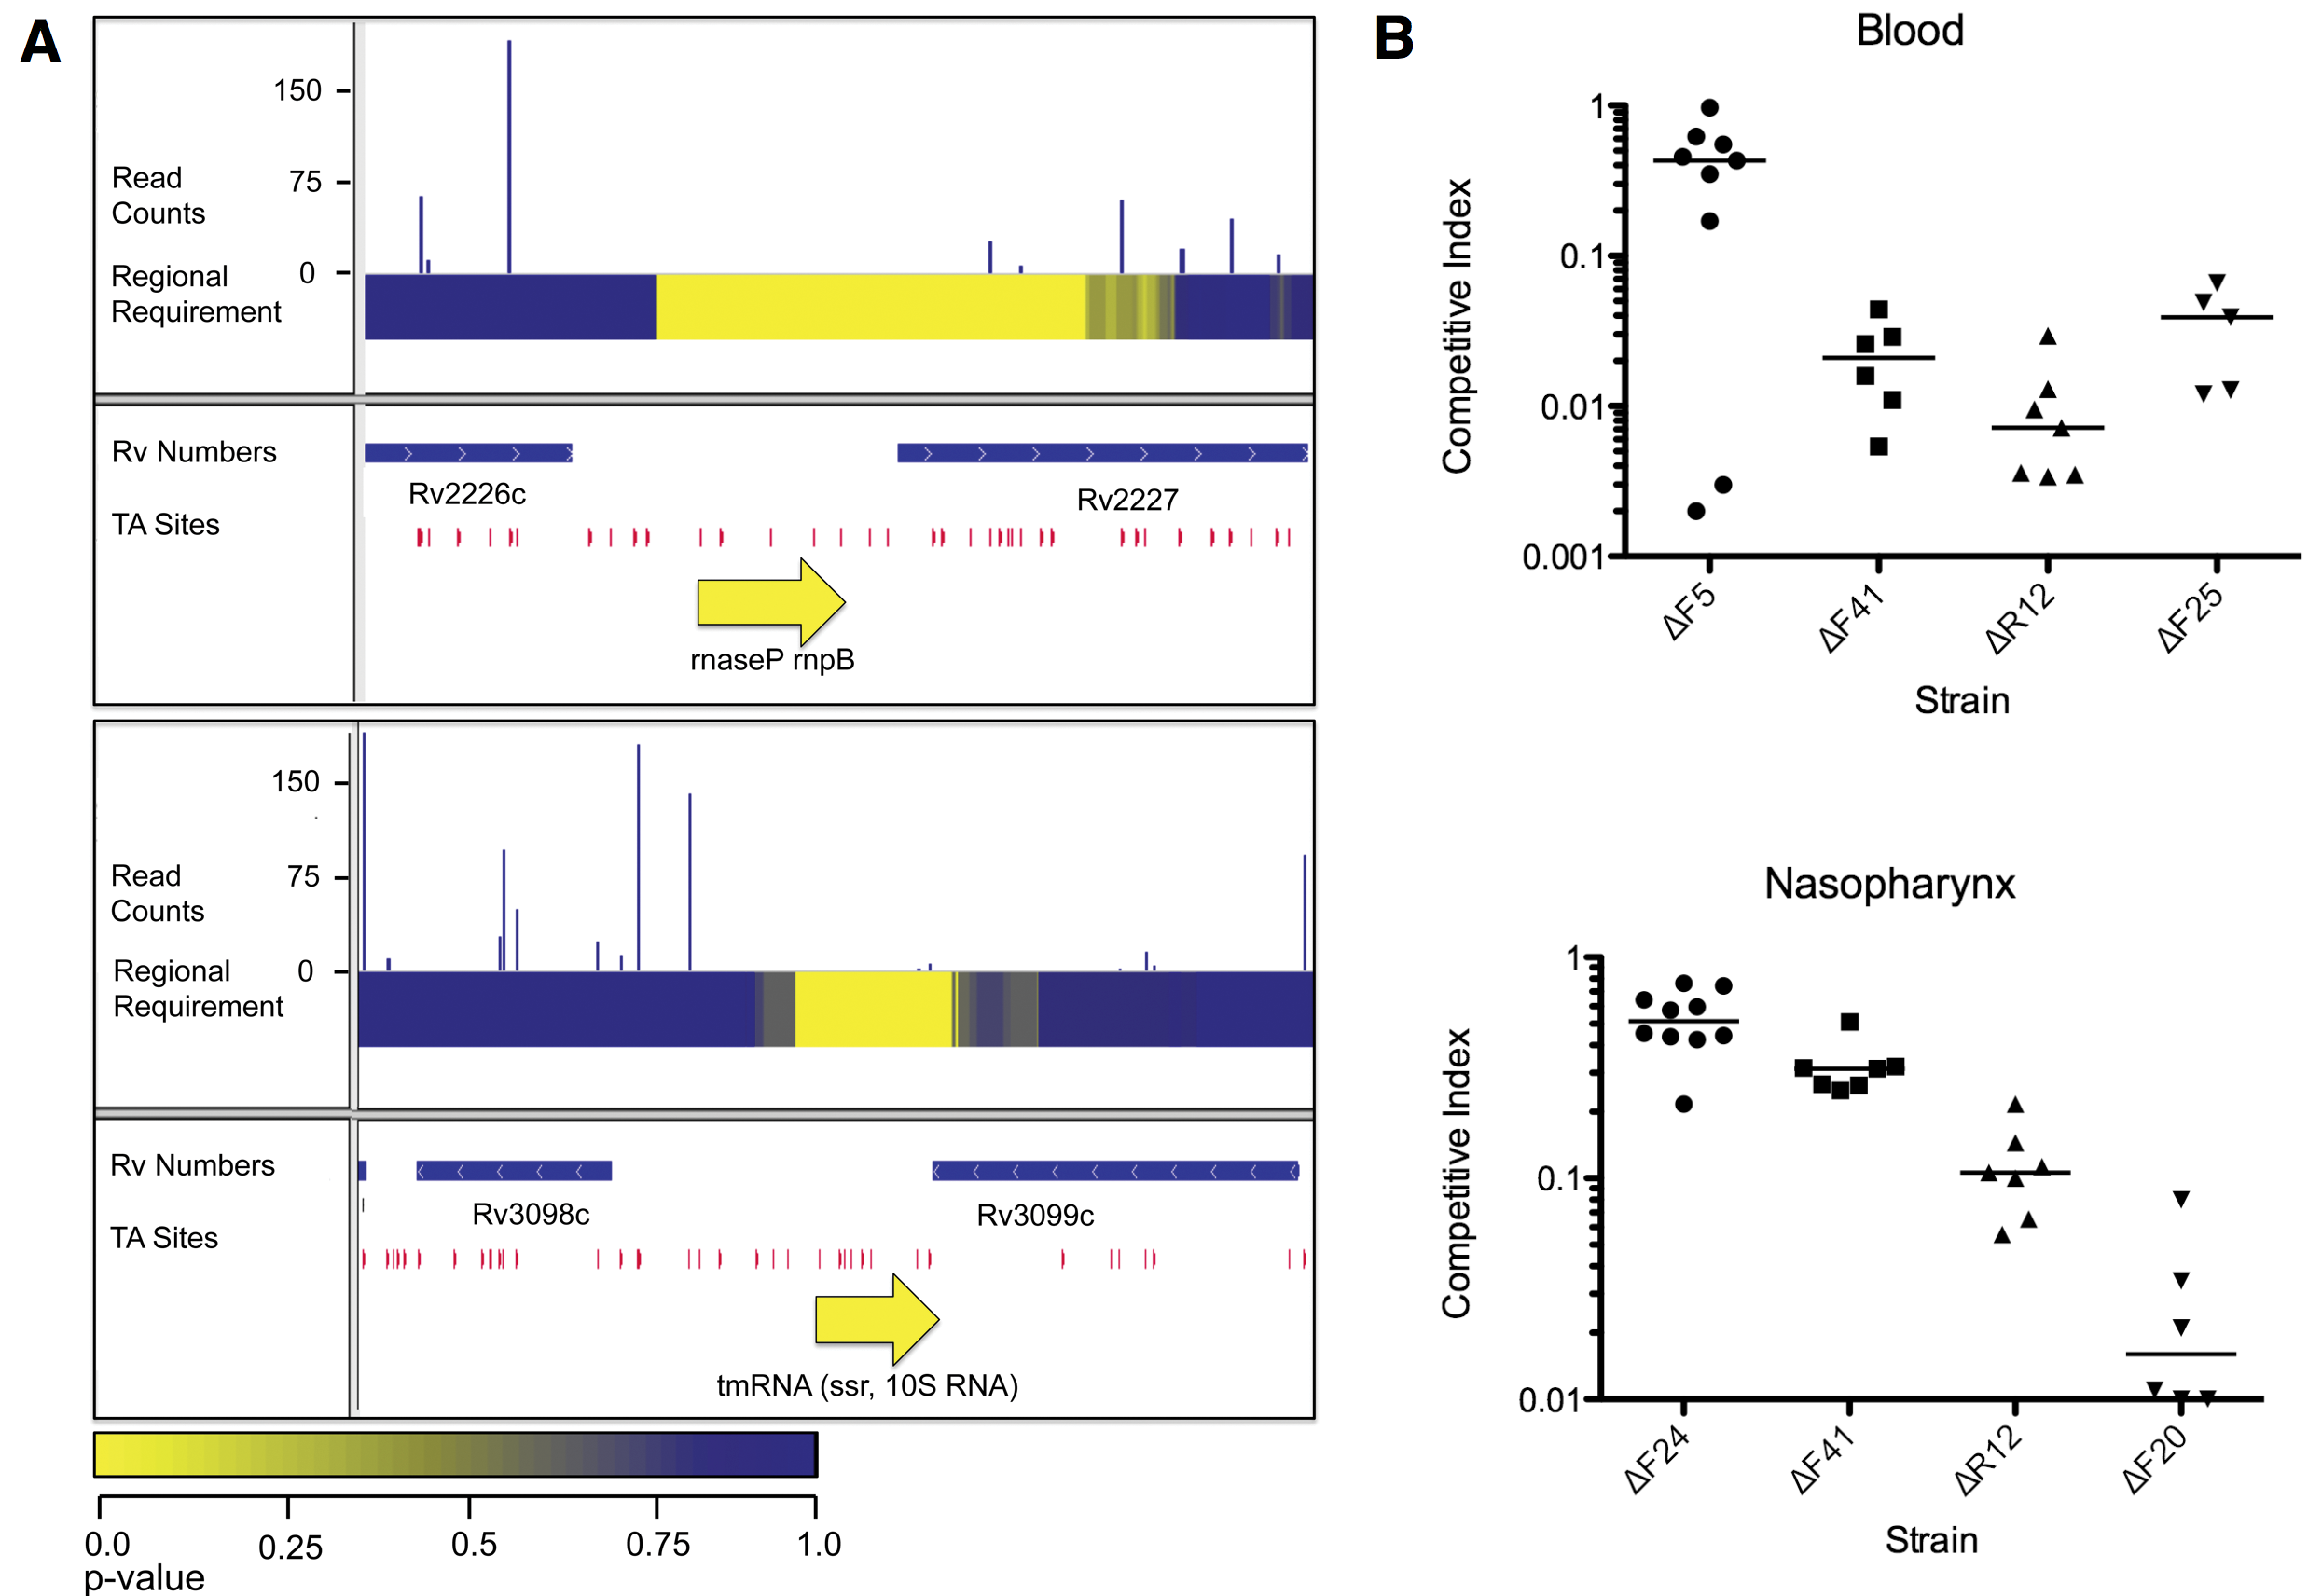
\includegraphics[width=14cm]{ncrnas.png}
\caption[Applications of transposon-insertion sequencing to non-coding RNAs]{\textbf{Applications of transposon-insertion sequencing to non-coding RNAs.} A) Plots of genomic regions in {\it Mycobacterium tuberculosis} containing the required non-coding RNAs RNase P (top) and tmRNA (bottom). Tracks, from top to bottom: 1. Histogram of insertion counts, 2. Comprehensive heat-map of requirement of 500-bp\nomenclature{bp}{Base pair} windows, 3. Position of annotated genes, 4. Position of TA dinucleotide sites, 5. Position of non-coding RNA. Reproduced from \textcite{Zhang2012}. B) 1 X 1 competition assays validate attenuating {\it Streptococcus pneumoniae} sRNA mutants identified by transposon-insertion sequencing. Mice were infected with defined deletions of sRNAs identified as attenuating by Tn-seq and wild type {\it S. pneumoniae} TIGR4 at the body site indicated and bacterial densities were compared 24 hours post-infection. These plots show the derived competitive index in blood (top) and the nasopharnyx (bottom). Each point represents the result of a competition experiment between an sRNA deletion mutant and wild-type TIGR4. A competitive index of 1 indicates equivalent numbers of mutants and wild-type were recovered. Modified from \textcite{Mann2012}.
} 
\label{fig:ncrnas}
\end{center}
\end{figure}

% Table generated by Excel2LaTeX from sheet 'Sheet1'
%
\begingroup
\begin{landscape}
   \tiny
   \noindent
    \begin{longtable}{ l
    				l
				l
				l
				p{2in}
				l
				l}
    \caption[Summary of transposon-insertion sequencing studies to date]{A collection of studies to date utilizing transposon-insertion sequencing. Columns: 1) study reference,  2) organism mutagenized, 3) number of mutants generated, 4) insertion density, 5) brief description of the application, 6) transposon used, 7) method name coined, if any.}
    \\
    \toprule
    \textbf{Study} & \textbf{Organism} & \textbf{Total Mutants} & \textbf{Density} & \textbf{Application} & \textbf{Tn used } & \textbf{Name Coined} \\
    \midrule
    \multirow{2}[1]{*}{\textcite{Hutchison1999}}  & \multirow{2}[1]{*}{\textit{M. genitalium}} & 1291  &  ~1/850 bp & \multirow{2}[1]{2in}{Required gene sets} & \multirow{2}[1]{*}{Tn4001} & \multirow{2}[1]{*}{GTM\nomenclature{GTM}{Global transposon mutagenesis} } \\
          &  \textit{M. pneumoniae}     & 918   & ~1/850 bp &       &       &  \\
    \multirow{2}[0]{*}{\textcite{Goodman2009}} & \multirow{2}[0]{*}{\textit{B. thetaiotaomicron}} & \multirow{2}[0]{*}{2 X 35,000} & \multirow{2}[0]{*}{1/182 bp} & \multirow{2}[0]{2in}{Establishment in human gut as a natural habitat} & \multirow{2}[0]{*}{Mariner} & \multirow{2}[0]{*}{INSeq} \\
          &       &       &       &       &       &  \\
    \multirow{2}[0]{*}{\textcite{Gawronski2009} } & \multirow{2}[0]{*}{\textit{H. influenzae}} & \multirow{2}[0]{*}{75,000} & \multirow{2}[0]{*}{1/32 bp} & \multirow{2}[0]{2in}{Prolonged survival in lung in vivo} & \multirow{2}[0]{*}{Mariner} & \multirow{2}[0]{*}{ HITS} \\
          &       &       &       &       &       &  \\
   \textcite{Opijnen2009}  & \textit{S. pneumoniae} & 6 x 25,000 & 1/91bp & Transcriptional regulation and carbohydrate transport & Mariner & Tn-seq \\
    \multirow{2}[0]{*}{\textcite{Langridge2009a}}  & \multirow{2}[0]{*}{{\it S.} Typhi1} & \multirow{2}[0]{*}{1.1 million} & 1/13 bp & \multirow{2}[0]{2in}{Gene requirements, bile tolerance} & \multirow{2}[0]{*}{Tn5} & \multirow{2}[0]{*}{TraDIS} \\
          &       &       &  &       &       &  \\
    \multirow{2}[0]{*}{\textcite{Gallagher2011}}  & \multirow{2}[0]{*}{\textit{P. aeruginosa}} & \multirow{2}[0]{*}{~100,000} & \multirow{2}[0]{*}{1/65 bp} & \multirow{2}[0]{2in}{Tobramycin resistance} & \multirow{2}[0]{*}{Mariner} & \multirow{2}[0]{*}{Tn-seq} \\
          &       &       &       &       &       & (circle method)  \\
    \textcite{Eckert2011}  & \textit{E. coli} & 19 x 95 & N/A & Colonization of bovine intestinal tract; retrospective re-evaluation of a STM study & Tn5   & - \\
    \textcite{Christen2011}  & \textit{C. crescentus} & 800,000 & 1/8bp & Gene/ncRNAs/promoter requirements & Tn5   & - \\
    \textcite{Griffin2011}  & \textit{M. tuberculosis} & 2 X 100,000 & 1/120bp & Gene requirements and cholesterol utilization & Mariner & - \\
    \textcite{Khatiwara2012}  & {\it S.} Typhimurium & 16,000 & ~1/610 & Bile, low nutrient and heat tolerance & Tn5   & - \\
    \textcite{Mann2012}  & \textit{S. pnuemoniae} & ~9,000-24,000 & Varying & Determining roles of sRNAs in pathogenesis & Mariner & - \\
    \textcite{Opijnen2012}  & \textit{S. pnuemoniae} & ~4,000 - 30,000 & Varying & Stress response and metabolism in vitro and murine in vivo colonization & Mariner & - \\
    \textcite{Brutinel2012} & \textit{S. oneidensis} & 50,000 &  ~1/191bp & Gene requirements and Metabolism & Mariner & - \\
    \textcite{Zhang2012} & \textit{M. tuberculosis} & 2 x 100,000 &  ~1/120 bp & Identifying genes, regulators and ncRNAs required for growth & Mariner & - \\
    \textcite{Klein2012}  & \textit{P. gingivalis} & N/A   & 1/43 bp & Gene requirements & Mariner & - \\
    \textcite{Pickard2013}  & {\it S.} Typhi1 & 1.1 million & 1/13 bp & Bacteriophage infection & Tn5   & - \\
    \multirow{2}[1]{*}{\textcite{Barquist2013a}}  & {\it S.} Typhi1 & 1.1million & 1/13 bp & \multirow{2}[1]{2in}{Comparison of gene requirements between two Salmonella serovars} & \multirow{2}[1]{*}{Tn5} & \multirow{2}[1]{*}{-} \\
          & {\it S.} Typhimurium & 930,000 & 1/9 bp &       &       &  \\
    \bottomrule
    \label{tab:studies}%
    \end{longtable}%
\end{landscape}%
\endgroup



While the non-coding transcripts of {\it M. tuberculosis} have been explored more thoroughly than those of {\it C. crescentus}, most remain functionally uncharacterized, though there are hints that some of these may be involved in pathogenicity \parencite{Arnvig2012}. Using a Mariner transposon-based assay and a windowed statistical analysis that accounted for the distribution of potential TA integration sites, 35 intergenic regions were identified as putatively required in the {\it M. tuberculosis} genome \parencite{Zhang2012}.  In common with the {\it C. crescentus} study, the RNA component of RNase P, required for the maturation of tRNAs, and tmRNA, involved in the freeing of stalled ribosomes, were identified as required (Figure \ref{fig:ncrnas} A) together with 10 non-redundant tRNAs and potential promoter regions. However, due to the lower overall insertion density and lack of TA sites in some GC-rich regions, there were some regions that could not be assayed and the resolution was limited to 250 bases.

A recent study has examined ncRNA requirements in the {\it S. enterica} serovars Typhi and Typhimurium \parencite{Barquist2013a}. Using the tRNAs as a model set of ncRNAs, this study showed that the high transposon insertion density achieved by the TraDIS protocol is capable of assaying the requirement for genomic regions as small as 70 to 80 bases. {\it S. enterica}, together with the closely related {\it E. coli}, has served as a model organism for the discovery and elucidation of ncRNA function, and extensive annotations of non-coding transcripts are available \parencite{Kroger2012, Burge2013, Raghavan2011,Chinni2010}. As a result this study was able to assay approximately 300 non-coding regions with evidence for function or transcription. Among the ncRNAs identified as required were RNase P; the RNA component of the signal recognition particle, involved in targeting proteins to the plasma membrane; and a number of known autoregulatory ribosomal protein leader sequences \parencite{Fu2013}, as well as providing evidence for a novel leader sequence, StyR-8 \parencite{Chinni2010}, that appears to be involved in the autoregulation of the {\it rpmB} gene. In total, this study identified 15 confirmed and putative ncRNAs required for robust competitive growth on rich media in both serovars, including a number of known sRNAs involved in stress response.

A particularly exciting study has been conducted in {\it S. pneumoniae} TIGR4 combining RNA-seq\nomenclature{RNA-seq}{RNA sequencing} with transposon-insertion sequencing \parencite{Mann2012}. To identify sRNA loci the authors first sequenced size-select RNA from the wild type and three two-component system knockouts, identifying 89 putative sRNAs, 56 of which were novel. Fifteen of these candidates, selected on the basis of high expression and low predicted folding free energy, were assayed for their ability to establish invasive disease in a murine model. Of these 8 sRNA deletions showed a significant attenuation of disease. To more broadly establish the roles of sRNAs in infecting particular organs, transposon insertion libraries were administered directly to the nasopharnyx, lungs, or blood of mice, and bacteria were harvested following disease progression. Twenty-six, 28, and 18 sRNAs were found to attenuate infection in the nasopharnyx, lung and blood respectively. These results were then validated with targeted deletions of 11 sRNAs (Figure  \ref{fig:ncrnas} B). In addition to establishing the role of sRNAs in {\it S. pneumoniae} virulence, this study illustrated the power of combining RNA-seq and transposon-insertion sequencing to rapidly assign phenotypes to non-coding sequences.

\section{Limitations}

In this review, we have largely focused on the potential of transposon insertion sequencing. However, this technology does have a number of important limitations, which we collect here and summarize in Table 2. As discussed previously, requirements for particular nucleotides at insertion sites, such as the TA required by Mariner transposons, or preference for certain sequence composition, such as the AT bias exhibited by Tn{\it 5}, can limit the density of observed insertions in certain genomic regions. This may impact any down-stream analysis, and can potentially bias results, particularly the determination of gene requirements. Even if this bias has been accounted for, transposon-insertion screens will always over-predict gene requirements in comparison to targeted deletion libraries as discussed previously. However, this over-prediction can be controlled either through careful consideration of known insertion biases as in many Mariner-based studies, or by high insertion densities, such as those achieved in several Tn{\it 5}-based studies (Table \ref{tab:studies}). Once the library has been created, only regions that have accumulated insertions in the conditions of library creation will be able to be assayed for fitness effects in further conditions. This means that regions that lead to slow growth phenotypes when disrupted in standard laboratory conditions may be difficult to assay in other conditions. Additionally, the dynamic range of fitness effects detected will depend on the complexity of the input library(s). The absence of insertions may be a particular problem for assaying small genomic elements, such as sRNAs or short ORFs\nomenclature{ORF}{Open reading frame}. Finally, the validation of hypotheses derived from transposon-insertion sequencing will require the construction of targeted deletions, as individual mutants cannot be recovered from pools unless specialized protocols have been followed during library construction (as in \cite{Goodman2009}).

\section{The future of transposon-insertion sequencing}

Transposon-insertion sequencing is a robust and powerful technique for the rapid connection of genotype to phenotype in a wide range of bacterial species. Already, a number of studies have demonstrated the effectiveness of this method and the results have been far-reaching: enhancing our understanding of basic gene functions, establishing requirements for colonization and infection, mapping complex metabolic pathways, and exploring non-coding genomic �dark matter�. Due to the range of potential applications of transposon-insertion sequencing, along with the decreasing cost and growing accessibility of next-generation sequencing, we believe that this method will become increasingly common in the near future. 

A number of bacterial species have already been subjected to transposon-insertion sequencing (Table \ref{tab:studies}). Microarray-based approaches to monitoring transposon mutant libraries have even been applied to eukaryotic systems(47), and similarly transposon-insertion sequencing can potentially be applied to any system where the creation of large-scale transposon mutant libraries is technologically feasible. Recently the Genomic Encyclopedia of Bacteria and Archea (GEBA)\nomenclature{GEBA}{Genomic encyclopedia of bacteria and archea} \parencite{Wu2009} has been expanding our knowledge of bacterial diversity through targeted genomic sequencing of underexplored branches of the tree of life. Applying transposon-insertion sequencing in a comparative manner \parencite{Barquist2013a} across the bacterial phylogeny will provide an unprecedented view of the determinants for survival in diverse environments. While most transposon-insertion sequencing studies to date have focused on pathogenic bacteria, these techniques could also have applications in energy production, bioremediation, and synthetic biology.

The combination of transposon-insertion sequencing with other high-throughput and computational methods is already proving to be fertile ground for enhancing our understanding of bacterial systems. For instance, by using transposon-insertion sequencing in a collection of relatively simple conditions combined with a computational pathway analysis, van Opijnen and Camilli were able to provide a holistic understanding of the genetic subsystems involved in a complex process such as {\it S. pneumoniae} pathogenesis. In the future, methods to assay phenotype in a high-throughput manner \parencite{Bochner2009,Nichols2011} may be combined with transposon-insertion sequencing to provide exhaustive simple genotype-phenotype associations with which to understand complex processes in a systems biology framework. We look forward to the adoption of these data sets by the community as an important tool for rapid hypothesis generation.

% ------------------------------------------------------------------------


%%% Local Variables: 
%%% mode: latex
%%% TeX-master: "../thesis"
%%% End: 



% \pagebreak[4]
% \hspace*{1cm}
% \pagebreak[4]
% \hspace*{1cm}
% \pagebreak[4]
%\usepackage[round,colon,authoryear]{natbib}

\chapter{A comparison of dense transposon insertion libraries in the \textit{Salmonella} serovars Typhi and Typhimurium}
\label{sec:chapterPingpong}
\ifpdf
    \graphicspath{{Chapter2/Chapter2Figs/EPS/}{Chapter2/Chapter2Figs/}}
\fi

\textit{This chapter is a modified version of the previously published article ``A comparison of dense transposon insertion libraries in the \emph{Salmonella} serovars Typhi and Typhimurium'' \parencite{Barquist2013a}. This work is a result of collaboration with Gemma C. Langridge (Pathogen Genomics, Wellcome Trust Sanger Institute), who constructed the \emph{Salmonella} Typhimurium transposon mutant library and contributed to a draft manuscript. In particular, portions of sections 2.3.1-3 have their genesis in \textcite{Langridge2010}, though have been significantly elaborated on here.}

\section{Introduction}

\textit{Salmonella enterica} subspecies \textit{enterica} serovars Typhi ({\it S.} Typhi) and Typhimurium ({\it S.} Typhimurium) are important, closely related, human pathogens with distinctly different lifestyles. In this chapter, I describe a study comparing dense transposon insertion libraries created in these two serovars. The results of this study demonstrate that orthologous genes can have dramatically different effects on the fitness of recently diverged organisms in rich media. These differences in fitness effects are indicative of changes in the network architecture of the cell which may partially underlie the dramatically different diseases caused by each organism and their different host ranges. Additionally, {\it S.} Typhimurium has served as a model organism for the discovery and functional characterization of ncRNAs. Comparing ncRNA requirements between it and a closely related serovar provides a glimpse of the functional evolution of non-coding regulatory networks.

\subsection{The genus {\it Salmonella}}

\textit{Salmonella} is a Gram-negative, $\gamma$-proteobacterial genus within the order Enterobacteriales, consisting of two species: \textit{Salmonella enterica} and \textit{Salmonella bongori}. Based on phylogenetic analyses of 16S and conserved amino acid sequences, it is most closely related to the genuses \textit{Escherichia}, \textit{Shigella}, and \textit{Citrobacter} \parencite{Paradis2005, Pham2007}. Molecular clock analyses suggest that \textit{Salmonella} and \textit{Escherichia} shared a common ancestor between 100 and 160 million years ago \parencite{Ochman1987, Doolittle1996}. During the time since their divergence \textit{Escherichia} has become established as a mammalian gut commensal, though multiple independent origins of the \textit{Shigella} and other pathogenic phenotypes within the genus show that a disease phenotype can be developed fairly easily through the horizontal acquisition of virulence determinants and the silencing of anti-virulence loci \parencite{Kaper2004,Prosseda2012}. On the other hand, despite sharing approximately 85\% of their genomes with \textit{Escherichia} and having broadly similar metabolic capabilities \parencite{AbuOun2009}, the \textit{Salmonellae} exist primarily as pathogens in mammals.

\begin{figure}[htp]
\begin{center}
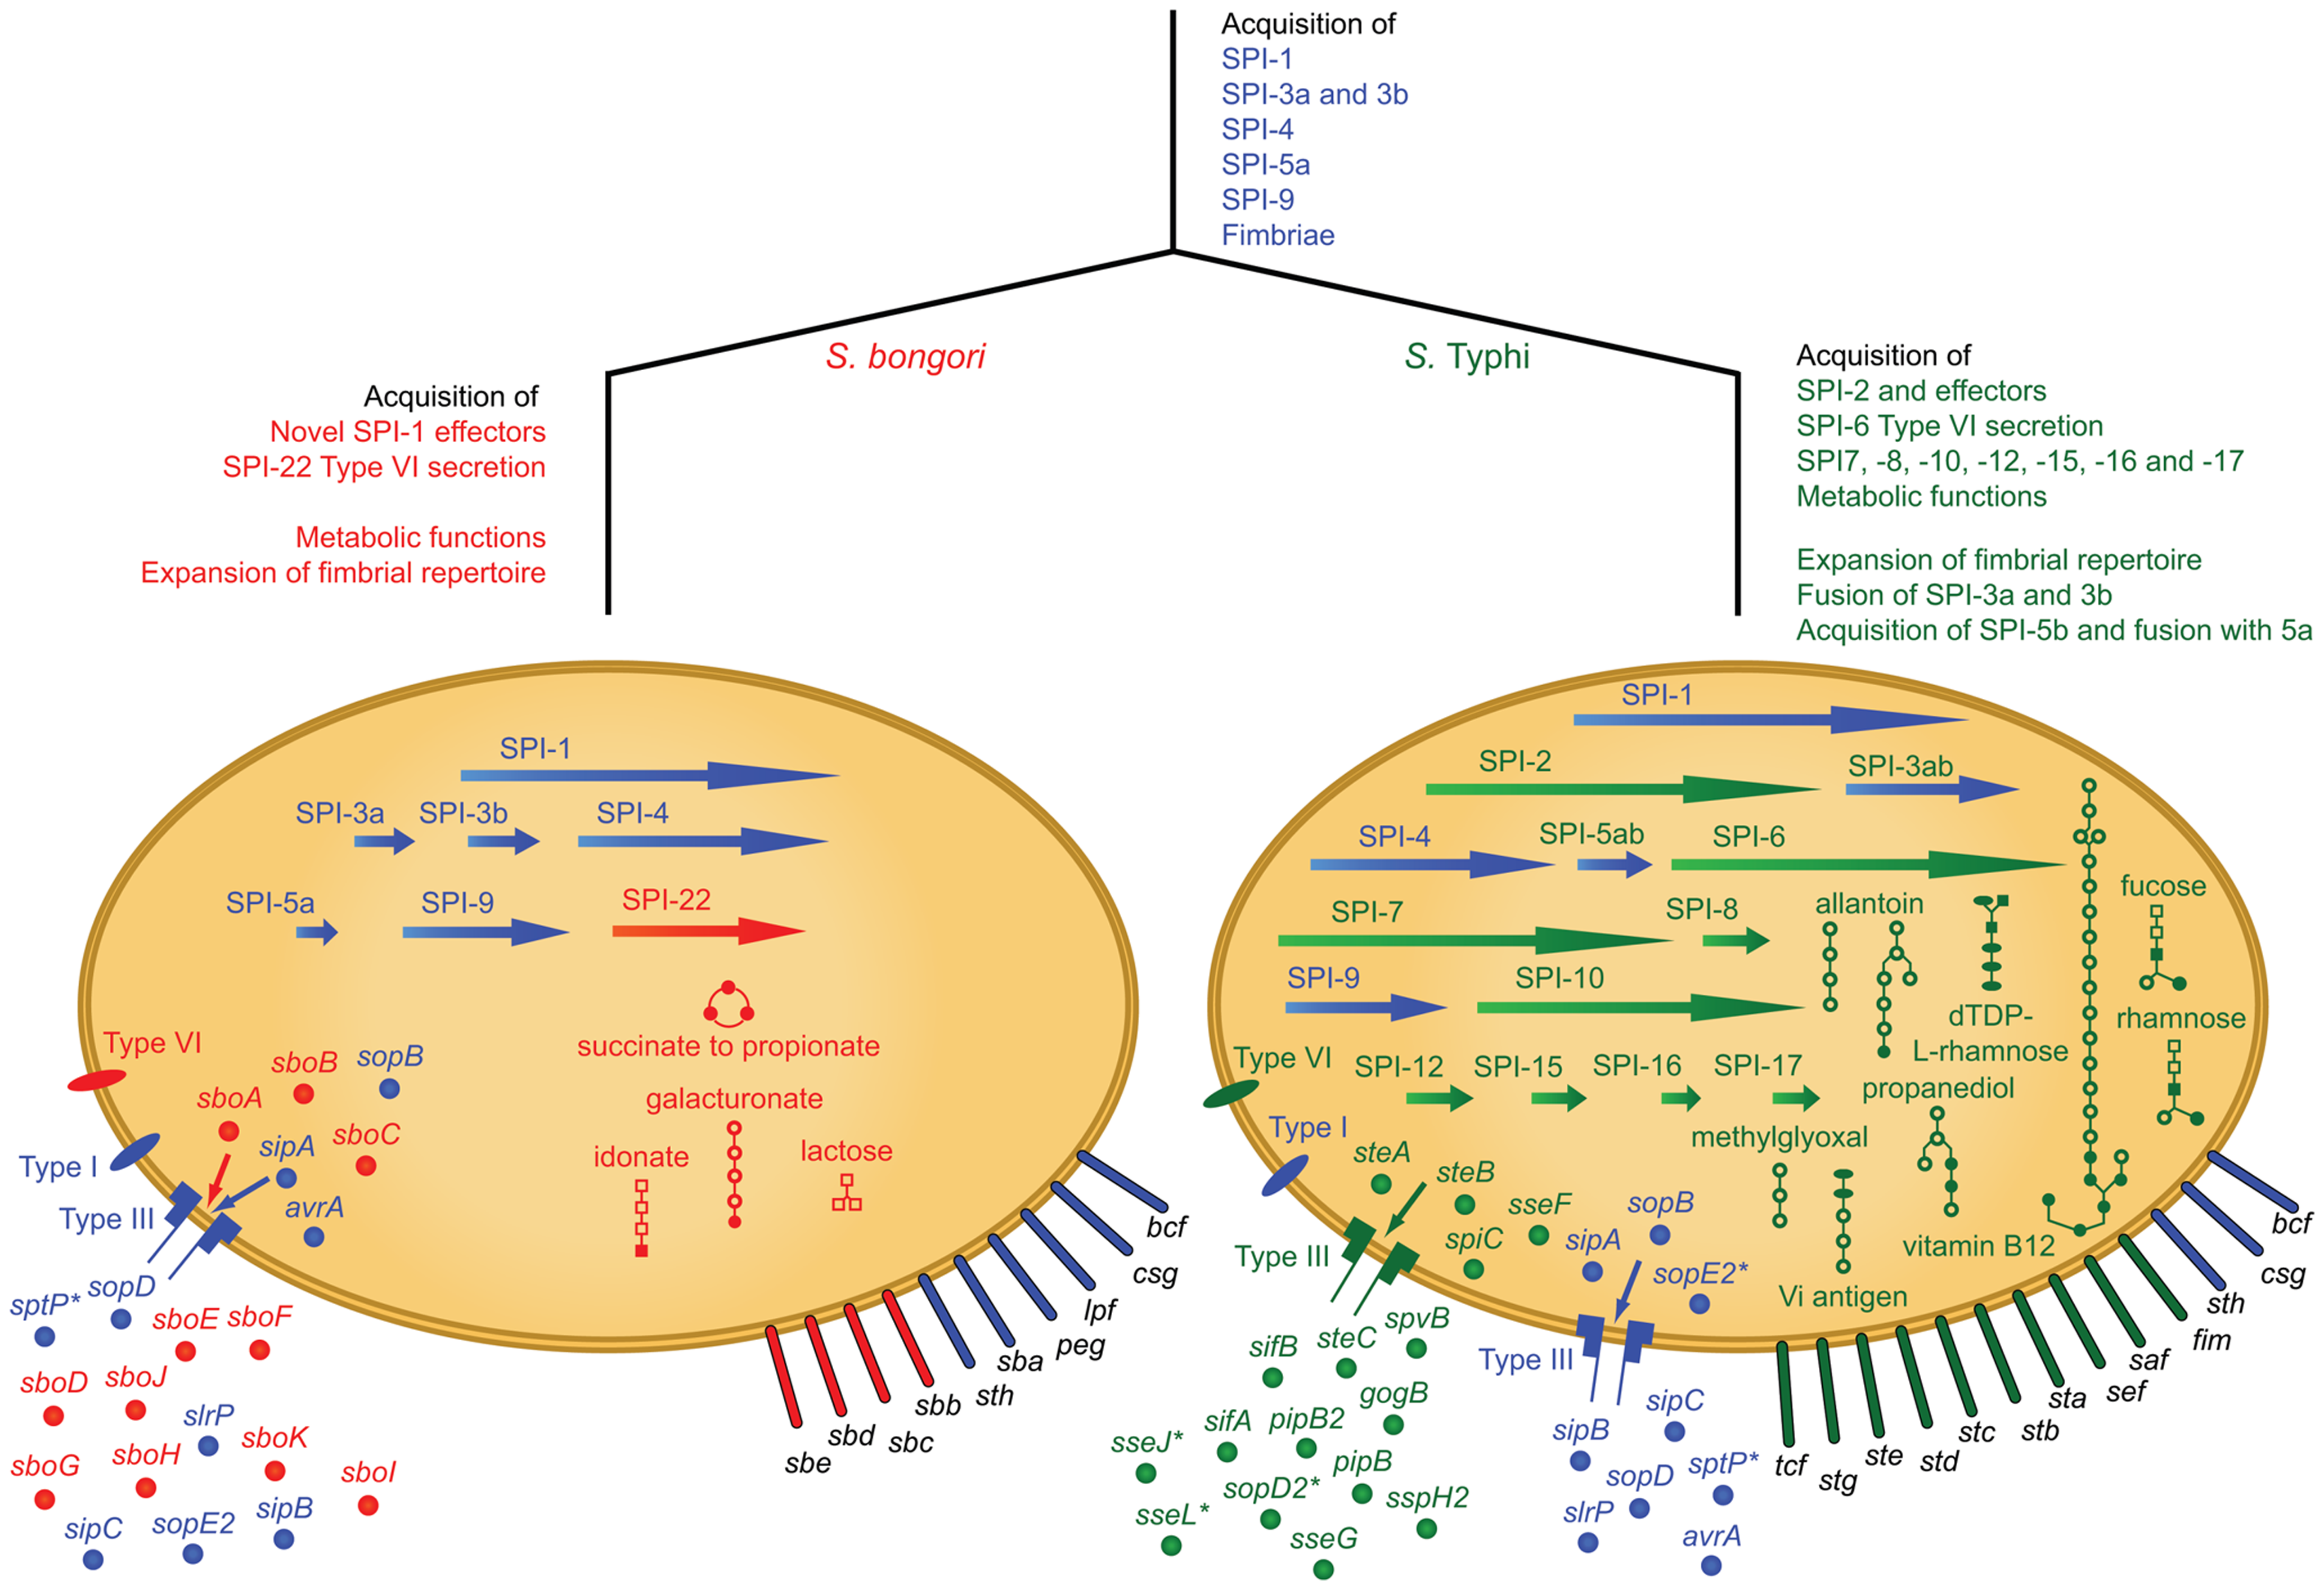
\includegraphics[width=14cm]{bongori.png}
\caption[Genomic acquisitions in the evolution of the \textit{Salmonellae}]{\textbf{Genomic acquisitions in the evolution of the \textit{Salmonellae}.} Traits shared by the common ancestor are depicted in blue; those unique to S. bongori are shown in red and those unique to S. Typhi in green. Arrows, Salmonella Pathogenicity Islands (SPIs); extended ovals, fimbriae; circles, effectors; small ovals and needle complexes, secretion systems. Metabolic pathways: lines, enzymatic reactions; open squares, carbohydrates; ovals, pyrimidines; open circles, other substrates; filled shapes, phosphorylated. Novel effectors acquired by S. bongori are secreted by the type III secretion system encoded on SPI-1. SPI-3a and 3b carry the same genes in both organisms but are fused into one island in S. Typhi. SPI-5a also carries the same genes in both organisms, but a further 3 kb (termed SPI-5b) has fused to SPI-5a in S. Typhi. *indicates a pseudogene. Reproduced from \parencite{Fookes2011}. 
} 
\label{fig:bongori}
\end{center}
\end{figure}

This difference in phenotype appears to be largely due to the acquisition of new virulence determinants which opened new niches to ancestral \textit{Salmonellae} (see figure \ref{fig:bongori}). Many of these determinants are encoded on large genomic islands with sizes between $\sim$6 and 140 kilobases termed \textit{Salmonella} Pathogenicity Islands (SPIs) \parencite{Hensel2004}. These islands encode a diverse array of virulence-related functions, including secretion systems, toxins, antibiotic resistances, and lipopolysaccharide (LPS)\nomenclature[Z]{LPS}{Lipopolysaccharide} and capsular modifications. In particular, the acquisition of SPI-1, encoding a type 3 secretion system (T3SS), and various fimbriae by the ancestral \textit{Salmonella} likely enabled invasion of cells in the intestinal epithelium and escape from competition with other members of the gut microbiota \parencite{Baumler1997}. \textit{S. bongori} appears to have only acquired a single addition SPI since its divergence from \textit{S. enterica} and likely retains a lifestyle more similar to the ancestral \textit{Salmonella}, though there is evidence for additional adaptation to its niche in the reptilian gut \parencite{Fookes2011}. \textit{S. enterica} meanwhile has diversified in to 6 distinct subspecies: {\it enterica}, {\it salamae}, {\it arizonae},{\it diarizonae}, {\it houtenae}, and {\it indica}. The acquisition of SPI-2, an enabling factor for systemic infection, by the ancestral {\it S. enterica} is thought to have been a driving force in this diversification \parencite{Baumler1997}. These subspecies are further divided in to over 2000 serovars based on the cell-surface O, flagellar H, and capsular Vi antigens \parencite{Grimont2007}. Subspecies besides {\it enterica} are thought to be primarily restricted to cold-blooded animals \parencite{Baumler1997}, though sporadic reports of zoonotic disease in mammals show these subspecies are capable of transiently colonizing the mammalian gut under certain conditions \parencite{Hilbert2012}. However, here I will be primarily concerned with subspecies {\it enterica} and its adaptation to the mammalian, and more specifically human, host.

\subsection{Host adaptation and restriction}

\subsection{Serovars Typhi and Typhimurium}
\textit{Salmonella enterica} subspecies \textit{enterica} serovars Typhi ({\it S.} Typhi) and Typhimurium ({\it S.} Typhimurium) are important human pathogens with distinctly different lifestyles. {\it S.} Typhi is host-restricted to humans and causes typhoid fever. This potentially fatal systemic illness affects at least 21 million people annually, primarily in developing countries \parencite{Crump2004, Bhutta2009, Kothari2008} and is capable of colonizing the gall bladder creating asymptomatic carriers; such individuals are the primary source of this human restricted infection, exemplified by the case of ``Typhoid Mary'' \parencite{Soper1939}. {\it S.} Typhimurium, conversely, is a generalist, infecting a wide range of mammals and birds in addition to being a leading cause of foodborne gastroenteritis in human populations. Control of {\it S.} Typhimurium infection in livestock destined for the human food chain is of great economic importance, particularly in swine and cattle \parencite{CDC2009, Majowicz2010}. Additionally, {\it S.} Typhimurium causes an invasive disease in mice, which has been used extensively as a model for pathogenicity in general and human typhoid fever specifically \parencite{Santos2001}.

Despite this long history of investigation, the genomic factors that contribute to these differences in lifestyle remain unclear. Over 85\% of predicted coding sequences are conserved between the two serovars in sequenced genomes of multiple strains \parencite{McClelland2001, Parkhill2001, Holt2008, Deng2003}. The horizontal acquisition of both plasmids and pathogenicity islands during the evolution of the salmonellae is believed to have impacted upon their disease potential. A 100kb plasmid, encoding the {\it Salmonella} plasmid virulence (SPV)\nomenclature[Z]{SPV}{{\it Salmonella} plasmid virulence (genes)} genes, is found in some {\it S.} Typhimurium strains and contributes significantly towards systemic infection in animal models \parencite{Gulig1987, Gulig1993}. {\it S.} Typhi is known to have harbored IncHI1 plasmids conferring antibiotic resistance since the 1970�s \parencite{Phan2009}, and there is evidence that these strains present a higher bacterial load in the blood during human infection \parencite{Wain1998}. Similar plasmids have been isolated from {\it S.} Typhimurium \parencite{Datta1962,Holt2007,Cain2012}. {\it Salmonella} pathogenicity islands (SPI)-1 and -2 are common to both serovars, and are required for invasion of epithelial cells (reviewed in \textcite{Darwin1999}) and survival inside macrophages respectively \parencite{Ochman1996,Shea1996}. {\it S.} Typhi additionally incorporates SPI-7 and SPI-10, which contain the Vi surface antigen and a number of other putative virulence factors \parencite{Pickard2003,Seth-Smith2008,Townsend2001}. 

Acquisition of virulence determinants is not the sole explanation for the differing disease phenotypes displayed in humans by {\it S.} Typhimurium and {\it S.} Typhi; genome degradation is an important feature of the {\it S.} Typhi genome, in common with other host-restricted serovars such as {\it S.} Paratyphi A (humans) and {\it S.} Gallinarum (chickens). In each of these serovars, pseudogenes account for 4-7\% of the genome \parencite{Parkhill2001,Thomson2008, Holt2009, McClelland2004}. Loss of function has occurred in a number of {\it S.} Typhi genes that have been shown to encode intestinal colonisation and persistence determinants in {\it S.} Typhimurium \parencite{Kingsley2003}. Numerous sugar transport and degradation pathways have also been interrupted \parencite{Parkhill2001}, but remain intact in {\it S.} Typhimurium, potentially underlying the restricted host niche occupied by {\it S.} Typhi.

In addition to its history as a model organisms for pathogenicity, {\it S.} Typhimurium has recently served as a model organism for the elucidation of non-coding RNA (ncRNA) function \parencite{Vogel2009a}. These include cis-acting switches, such as RNA-based temperature and magnesium ion sensors \parencite{Waldminghaus2007, Cromie2006}, together with a host of predicted metabolite-sensing riboswitches. Additionally, a large number of trans-acting small RNAs (sRNAs) have been identified within the {\it S.} Typhimurium genome \parencite{Kroger2012}, some with known roles in virulence \parencite{Hebrard2012}. These sRNAs generally control a regulon of mRNA transcripts through an antisense binding mechanism mediated by the protein Hfq in response to stress. The functions of these molecules have generally been explored in either {\it S.} Typhimurium or {\it E. coli}, and it is unknown how stable these functions and regulons are over evolutionary time \parencite{Richter2012}.

Transposon mutagenesis has previously been used to assess the requirement of particular genes for cellular viability. The advent of next-generation sequencing has allowed simultaneous identification of all transposon insertion sites within libraries of up to 1 million independent mutants (reviewed in \textcite{Barquist2013}; see also the previous chapter), enabling us to answer the basic question of which genes are required for {\it in vitro} growth with extremely fine resolution. By using transposon mutant libraries of this density, which in {\it S.} Typhi represents on average $>$ 80 unique insertions per gene \parencite{Langridge2009a}, shorter regions of the genome can be interrogated, including ncRNAs \parencite{Christen2011}. In addition, once these libraries exist, they can be screened through various selective conditions to further reveal which functions are required for growth/survival.

Using Illumina-based transposon directed insertion-site sequencing (TraDIS \parencite{Langridge2009a}) with large mutant libraries of both {\it S.} Typhimurium and {\it S.} Typhi, we investigated whether these Salmonellae require the same protein-coding and non-coding RNA (ncRNA) gene sets for competitive growth under laboratory conditions, and whether there are differences which reflect intrinsic differences in the pathogenic niches these bacteria inhabit.

\section{Materials and Methods}

\subsection{Strains}
{\it S.} Typhimurium strain SL3261 contains a deletion relative to the parent strain, SL1344, was used to generate the large transposon mutant library. The 2166bp deletion ranges from 153bp within {\it aroA} (normally 1284bp) to the last 42bp of {\it cmk}, forming two pseudogenes and deleting the intervening gene SL0916 completely. For comparison, we utilized our previously generated {\it S.} Typhi Ty2 transposon library \parencite{Langridge2009a}.

\subsection{Annotation}
For {\it S.} Typhimurium strain SL3261, we used feature annotations drawn from the SL1344 genome (EMBL-Bank accession FQ312003.1), ignoring the deleted {\it aroA}, {\it ycaL}, and {\it cmk} genes. We re-analyzed our {\it S.} Typhi Ty2 transposon library with features drawn from an updated genome annotation (EMBL-Bank accession AE014613.1.) We supplemented the EMBL-Bank annotations with non-coding RNA annotations drawn from Rfam 10.1 \parencite{Burge2013}, \textcite{Sittka2008}, \textcite{Chinni2010}, \textcite{Raghavan2011}, and \textcite{Kroger2012}. Selected protein-coding gene annotations were supplemented using the HMMER webserver \parencite{Finn2011} and Pfam \parencite{Punta2012}.

\subsection{Creation of {\it S.} Typhimurium transposon mutant library}
{\it S.} Typhimurium was mutagenized using a Tn5-derived transposon as described previously (\cite{Langridge2009a}; a detailed protocol is available in \cite{Langridge2010}). Briefly, the transposon was combined with the EZ-Tn5 transposase (Epicenter, Madison, USA) and electroporated into {\it S.} Typhimurium. Transformants were selected by plating on LB agar containing 15 $\mu$g/mL kanamycin and harvested directly from the plates following overnight incubation. A typical electroporation experiment generated a batch of between 50,000 and 150,000 individual mutants. 10 batches were pooled together to create a mutant library comprising approximately 930,000 transposon mutants.

\subsection{DNA manipulations and sequencing}
Genomic DNA was extracted from the library pool samples using tip-100g columns and the genomic DNA buffer set from Qiagen (Crawley, UK). DNA was prepared for nucleotide sequencing as described previously \parencite{Langridge2009a}. Prior to sequencing, a 22 cycle PCR was performed as previously described \parencite{Langridge2009a}. Sequencing took place on a single end Illumina flowcell using an Illumina GAII sequencer, for 36 cycles of sequencing, using a custom sequencing primer and 2x Hybridization Buffer \parencite{Langridge2009a}. The custom primer was designed such that the first 10 bp of each read was transposon sequence.  

\subsection{Sequence analysis}
The Illumina FASTQ sequence files were parsed for 100\% identity to the $5'$ 10bp of the transposon (TAAGAGACAG). Sequence reads which matched were stripped of the transposon tag and subsequently mapped to the {\it S.} Typhimurium SL1344 or {\it S.} Typhi Ty2 chromosomes using Maq version maq-0.6.8 \parencite{Li2008}. Approximately 12 million sequence reads were generated from the sequencing run which used two lanes on the Illumina flowcell. Precise insertion sites were determined using the output from the Maq mapview command, which gives the first nucleotide position to which each read mapped. The number and frequency of insertions mapping to each nucleotide in the appropriate genome was then determined. 

\subsection{Statistical analysis of required genes}
The number of insertion sites for any gene is dependent upon its length, so the values were made comparable by dividing the number of insertion sites by the gene length, giving an ``insertion index'' for each gene. As before \parencite{Langridge2009a} the distribution of insertion indices was bimodal, corresponding to the required (mode at 0) and non-required models (See Figure \ref{fig:gamma}). We fitted gamma distributions for the two modes using the R MASS library (http://www.r-project.org). $Log_2$-likelihood ratios (LLR)\nomenclature[Z]{LLR}{$Log_2$-likelihood ratios} were calculated between the required and non-required models and we called a gene required if it had an LLR of less than -2, indicating it was at least 4 times more likely according to the required model than the non-required model. ``Non-required'' genes were assigned for an LLR of greater than 2. Genes falling between the two thresholds were considered ``ambiguous'' for the purpose of this analysis. This procedure lead to genes being called as required in {\it S.} Typhimurium when their insertion index was less than 0.020, and ambiguous between 0.020 and 0.027. The equivalent cut-offs for the {\it S.} Typhi library are 0.0147 and 0.0186, respectively.

\begin{figure}[htp]
\begin{center}
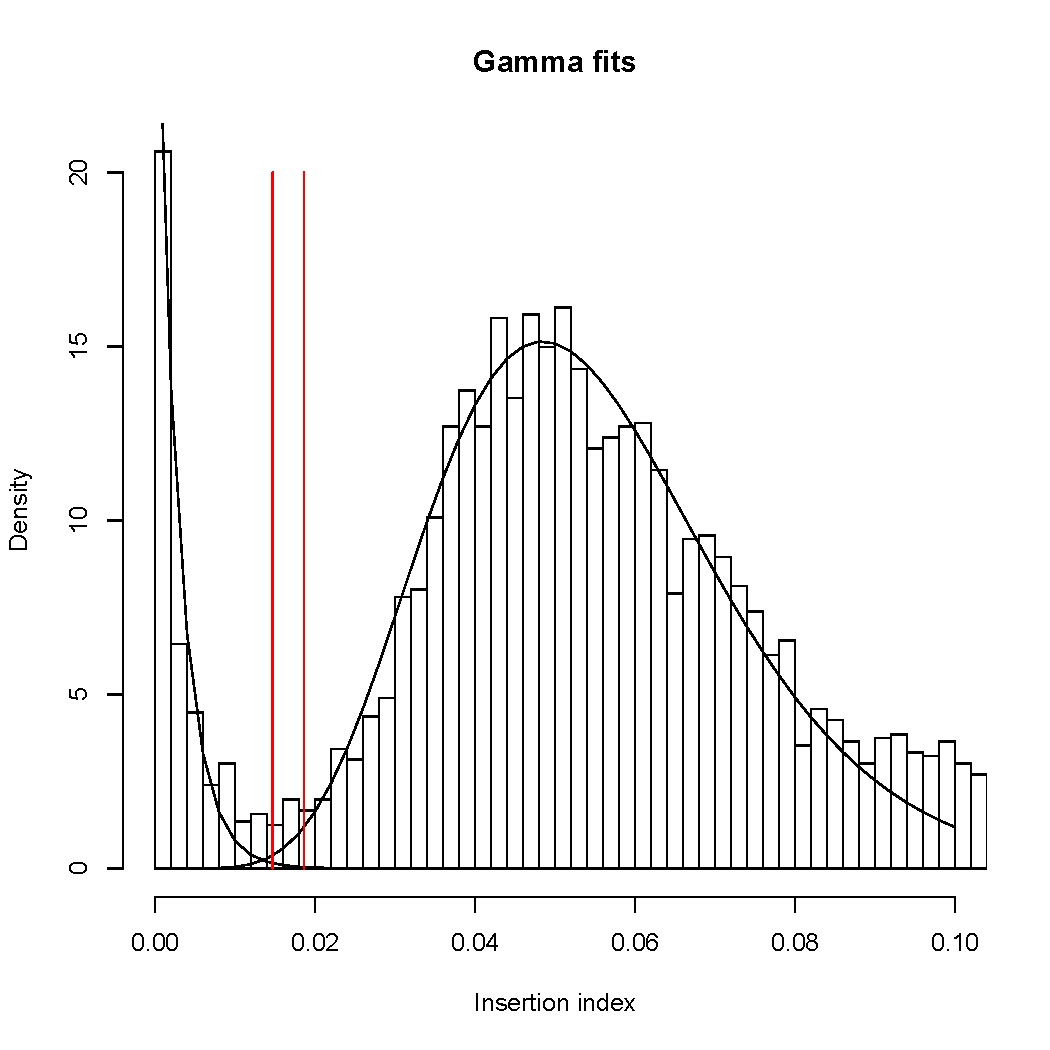
\includegraphics[width=14cm]{typhi_gamma}
\caption[The distribution of gene-wise insertion indexes in {\it S.} Typhi]{\textbf{The distribution of gene-wise insertion indexes in {\it S.} Typhi.} Bars report the density of genes with insertion indexes within each range, black lines show gamma distributions fitted to the required (left, mode at 0) and non-required (right) peaks, and red lines report associated LLR-based cut-offs for calling gene ambiguity (left) and requirement (right). The distribution of insertion indexes in {\it S.} Typhimurium is similar, though with a wider separation between the required and non-required peaks due to the higher insertion density attained. 
} 
\label{fig:gamma}
\end{center}
\end{figure}

We calculated a p-value for the observed number of insertion sites per gene using a Poisson approximation with rate $R = \frac{N}{G}$ where $N$ is the number of unique insert sites (549,086) and $G$ is the number of bases in the genome (4,878,012). The p-value for at least $X$ consecutive bases without an insert site is $e^{(-RX)}$, giving a 5\% cut-off at 27 bp and a 1\% cut-off at 41 bp.

For every gene $g$ with $n_{g,A}$ reads observed in {\it S.} Typhi and $n_{g,B}$ reads observed in {\it S.} Typhimurium, we calculated the log2 fold change ratio $S_{g,A,B} = log2 ((n_{g,A}+100)/(n_{g,B}+100))$. The correction of 100 reads smoothes out the high scores for genes with very low numbers of observed reads. We fitted a normal model to the mode +/- 2 sample standard deviations of the distribution of $S_{A,B}$, and calculated p-values for each gene according to the fit. We considered genes with a p-value of 0.05 or less under the normal model to be uniquely required by one serovar.

\section{Results and Discussion}

\subsection{TraDIS assay of every {\it Salmonella} Typhimurium protein-coding gene}
Approximately 930,000 mutants of {\it S.} Typhimurium were generated using a Tn5-derived transposon. 549,086 unique insertion sites were recovered from the mutant library using short-read sequencing with transposon-specific primers. This is a substantially higher density than the 371,775 insertions recovered from {\it S.} Typhi previously \parencite{Langridge2009a}. The {\it S.} Typhimurium library contains an average of one insertion every 9bp, or over 100 unique inserts per gene (figure  \ref{fig:genome}). The large number of unique insertion sites allowed every gene to be assayed; assuming random insertion across the genome, a region of 41bp without an insertion was statistically significant (P $<$ 0.01).  As previously noted in {\it S.} Typhi, the distribution of length-normalized insertions per gene is bimodal (see supplementary figure 1), with one mode at 0. We interpret genes falling in to the distribution around this mode as being required for competitive growth within a mixed population under laboratory conditions (hereafter ``required''). Of these, 57 contained no insertions whatsoever and were mostly involved in core cellular processes (see table \ref{tab:core}, Supplementary Dataset).

\begin{figure}[htp]
\begin{center}
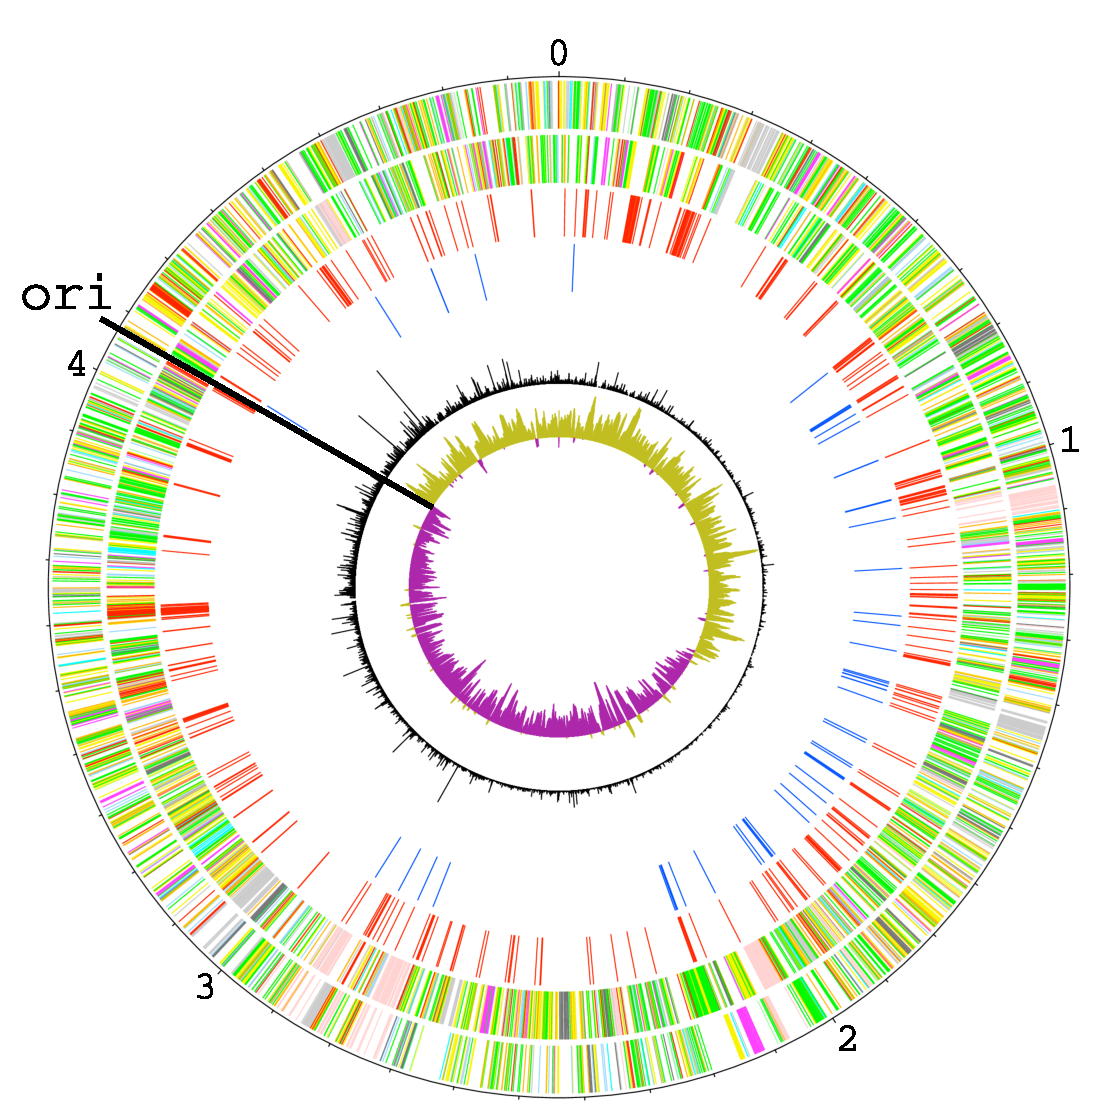
\includegraphics[width=14cm]{genome}
\caption[Genome-wide transposon mutagenesis of {\it S.} Typhimurium]{\textbf{Genome-wide transposon mutagenesis of {\it S.} Typhimurium.} A) Circular plot showing gene content, distribution of required genes, and insertion density along the {\it S.} Typhimurium chromosome. The outer scale is marked in megabases. Circular tracks range from 1 (outer track) to 6 (inner track). Track 1, all forward-strand genes (color-coded according to function: dark blue, pathogenicity/adaptation; black, energy metabolism; red, information transfer; dark green, membranes/surface structures; cyan, degradation of macromolecules; purple, degradation of small molecules; yellow, central/intermediary metabolism; light blue, regulators; pink, phage/IS elements; orange, conserved hypothetical; pale green, unknown function; brown, pseudogenes.); track 2, all reverse-strand genes (color-coded as for forward-strand genes); track 3, {\it S.} Typhimurium required genes (red); track 4, 56 genes required by {\it S.} Typhimurium but not by {\it S.} Typhi (dark blue, see also table 1); track 5, transposon insertion density; track 6, GC bias ((G-C)/(G+C)), khaki indicates values $>$1; purple $<$1.
} 
\label{fig:genome}
\end{center}
\end{figure}

There was a bias in the frequency of transposon insertion towards the origin of replication. This likely occurred as the bacteria were in exponential growth phase immediately prior to transformation with the transposon. In this phase of growth, multiple replication forks would have been initiated, meaning genes closer to the origin were in greater copy number and hence more likely to be a target for insertion. We also observed a bias for transposon insertions in A+T rich regions, as was previously observed in the construction of an {\it S.} Typhi mutant library \parencite{Langridge2009a}. However, the insertion density achieved is sufficient to discriminate between required and non-required genes easily. As was first seen in {\it S.} Typhi \parencite{Langridge2009a}, we observed transposon insertions into genes upstream of required genes in the same operon, suggesting that most insertions do not have polar effects leading to the inactivation of downstream genes.

Analysis of the {\it S.} Typhimurium mutant library allowed us to identify 353 coding sequences required for growth under laboratory conditions, and 4,112 non-required coding sequences (see Supplementary Dataset). We were unable to assign 65 genes to either the required or non-required category. 60 of these genes, which we will refer to as ``ambiguous'', had log-likelihood ratios (LLRs) between -2 and 2. The final 5 unassigned genes had lengths less than 60 bases, and they were removed from the analysis. All other genes contained enough insertions or were of sufficient length to generate credible LLR scores. Thus, every gene was assayed and we were able to draw conclusions for 98.7\% of the coding genome in a single sequencing run (figure \ref{fig:genome}).

\subsection{Cross-species comparison of genes required for growth}

\begin{figure}[htp]
\begin{center}
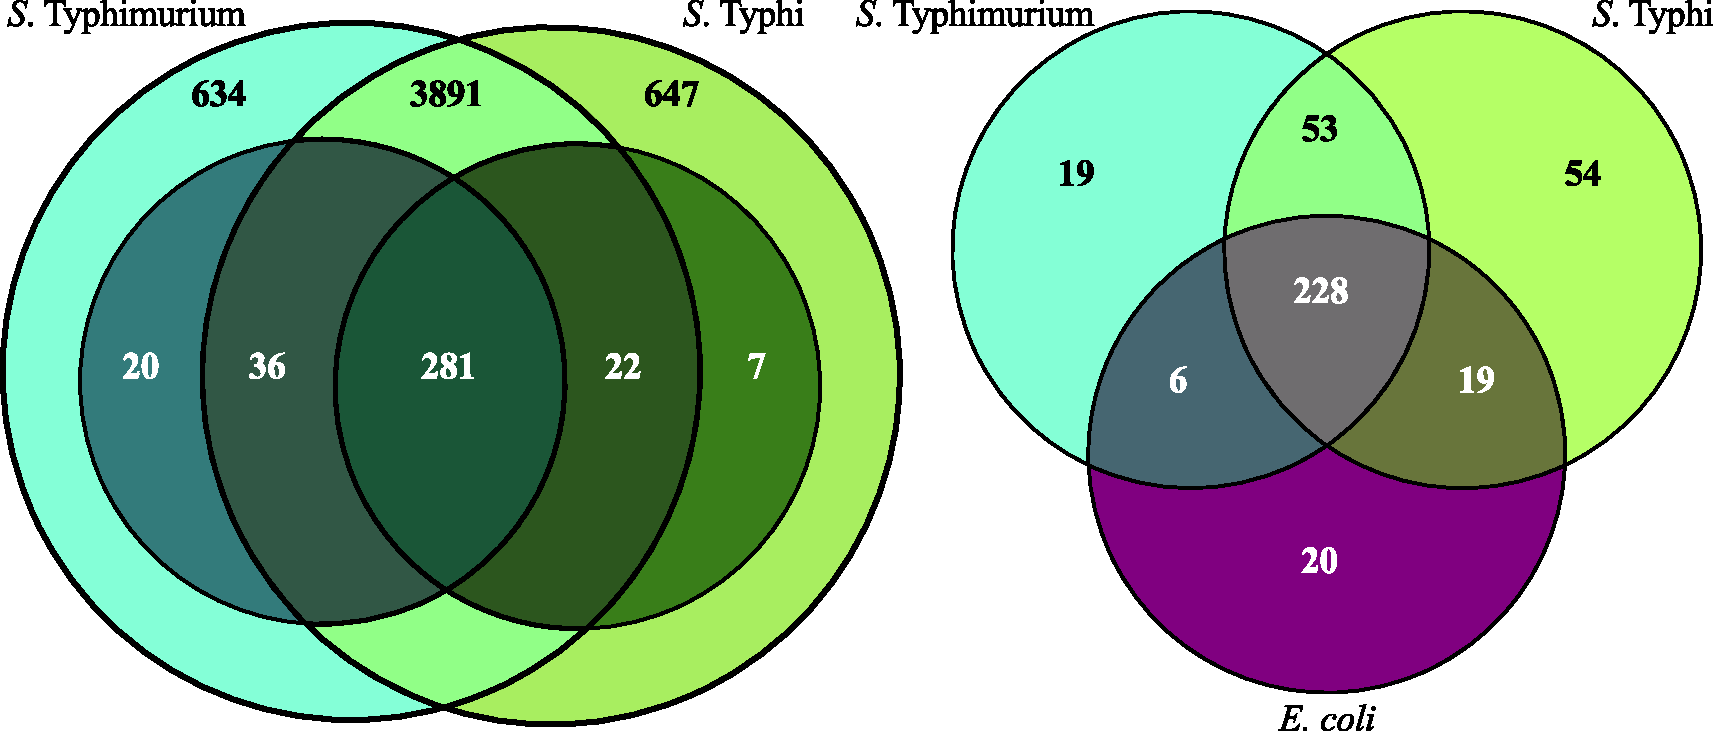
\includegraphics[width=14cm]{venn}
\caption[Comparison of required genes]{\textbf{Comparison of required genes.} Venn diagrams showing (A) the overlap of all genes (outer circles, light colors) and required genes (inner circles, dark colors) between {\it S.} Typhimurium and {\it S.} Typhi (excluding genes required in one serovar only which do not have significantly different read-counts). Black numbers refer to all genes, white numbers to required genes. (B) the overlap of all required genes between {\it S.} Typhimurium (blue), {\it S.} Typhi (green) and {\it E. coli} (purple). White numbers refer to genes with Keio essentiality scores $>=$ 0.5.
} 
\label{fig:venn}
\end{center}
\end{figure}

Gene essentiality has previously been assayed in {\it Salmonella} using insertion-duplication mutagenesis. \textcite{Knuth2004} estimated 490 genes are essential to growth in clonal populations, though 36 of these have subsequently been successfully deleted \parencite{Santiviago2009}. While TraDIS assays gene requirements after a brief period of competitive growth on rich media, we identify a smaller required set than \textcite{Knuth2004} of approximately 350 genes in each serovar, closer to current estimates of approximately 300 essential genes in {\it E. coli} \parencite{Baba2006}. 

To demonstrate that TraDIS does identify genes known to have strong effects on growth, as well as to test our predictive power for determining gene essentiality, we compared our required gene sets in {\it S.} Typhimurium and {\it S.} Typhi to essential genes determined by systematic single-gene knockouts in the {\it Escherichia coli} K-12 Keio collection \parencite{Baba2006}. We identified orthologous genes in the three data sets by best reciprocal FASTA\nomenclature[Z]{FASTA}{Fast alignment} hits exhibiting over 30\% sequence identity for the amino acid sequences. Required orthologous genes identified in this manner share a significantly higher average percent sequence identity with their {\it E. coli} counterparts than expected for a random set of orthologs, at $\sim$94\% identity as compared to $\sim$87\% for all orthologous genes. In 100,000 randomly chosen gene sets of the same size as our required set we did not find a single set where the average shared identity exceeded 90\%, indicating that required genes identified by TraDIS are more highly conserved at the nucleotide level than other orthologous protein coding sequences.

\textcite{Baba2006} have defined an essentiality score for each gene in {\it E. coli} based on evidence from four experimental techniques for determining gene essentiality: targeted knock-outs using $\lambda$-red\nomenclature[G]{$\lambda$}{Phage lambda} mediated homologous recombination, genetic footprinting \parencite{Gerdes2003,Tong2004}, large-scale chromosomal deletions \parencite{Hashimoto2005}, and transposon mutagenesis \parencite{Kang2004}.  Scores range from -4 to 3, with negative scores indicating evidence for non-essentiality and positive scores indicating evidence for essentiality. Comparing the overlap between essential gene sets in {\it E. coli}, {\it S.} Typhi, and {\it S.} Typhimurium, we find a set of 228 {\it E. coli} genes which have a Keio essentiality score of at least 0.5 (i.e. there is evidence for gene essentiality; See Figure \ref{fig:venn}.) that have TraDIS-predicted required orthologs in both {\it S.} Typhi and {\it S.} Typhimurium, constituting $\sim$85\% of E. coli genes with evidence for essentiality indicating that gene requirements are largely conserved between these genera. Including orthologous genes that are only predicted to be essential by TraDIS in {\it S.} Typhi or {\it S.} Typhimurium raises this figure to nearly 93\%. The majority of shared required genes between all three bacteria are responsible for fundamental cell processes, including cell division, transcription and translation. A number of key metabolic pathways are also represented, such as fatty acid and peptidoglycan biosynthesis (Table \ref{tab:core}). A recent study in the alphaproteobacteria {\it Caulobacter crescentus} reported 210 shared essential genes with {\it E. coli}, despite {\it C. crescentus} sharing less than a third as many orthologous genes with {\it E. coli} as {\it Salmonella} serovars \parencite{Christen2011}. This suggests the existence of a shared core of approximately 200 essential proteobacterial genes, with the comparatively rapid turnover of 150 to 250 �non-core� lineage-specific essential genes.  

% Table generated by Excel2LaTeX from sheet 'Sheet1'
%
\begin{landscape}
\begin{table}
   \small
   \centering
   \noindent
    \caption[Core genome functions in \emph{S.} Typhimurium]{\textbf{Core genome functions in \emph{S.} Typhimurium.} Protein-coding genes providing fundamental biological functions in \emph{S.} Typhimurium. Genes in bold are required in\emph{S.} Typhi (log-likelihood ratio (LLR) between required and non-required models $<$ -2; see Methods.) * indicates genes ambiguous in \emph{S.} Typhimurium, having a LLR between -2 and 2. }
    \begin{tabular}{     l
    				p{1.5in}
				p{2.9in}
				p{2in}
				}
   
    \\
    \toprule
    \textbf{Biological Process} & \textbf{Sub-process} & \textbf{Required genes} & \textbf{Non-required genes}\\
    \midrule
    Cell division & & \emph{\textbf{ftsALKQWYZ}, minE, mukB, SL2391} & \emph{\textbf{ftsHJNX}*, minCD, sdiA, cedA, sulA}\\
    DNA replications & Polymerases I, II, and III & \emph{\textbf{dnaENQX, holAB}} & \emph{\textbf{polA}B, holC\textbf{D}E}\\
    & Supercoiling & \emph{\textbf{gyrAB, parCE}} & \\
    & Primosome-associated & \emph{\textbf{dnaBCGT, priA, ssb}} & \emph{\textbf{priB}*C, \textbf{rep}}\\
    Transcription & RNA polymerase & \emph{\textbf{rpoABC}} & \\
    & Sigma, elongation, anti- and termination factors & \emph{\textbf{nusBG, rpoDH, rho}} & \emph{\textbf{nusA, rpoE}NS}\\
    Translation & tRNA-synthetases & \emph{\textbf{alaS, argS, asnS, aspS, cysS, glnS, gltX, glyQS, hisS, ileS, leuS, lysS, metG, pheST, proS, serS, thrS, tyrS, valS}} & \emph{trpS, trpS2}\\
    & Ribosome components & \emph{\textbf{rplBCDEFJKLMNOPQRSTUVWXY, rpmABCDHI, rpsABCDEFGHIJKLMNPQST}} & \emph{rplAI, rpmEE2, rpmFH\textbf{J}J2, rps\textbf{OR}*\textbf{U}*V} \\
    & Initiation, elongation, and peptide chain release factors & \emph{\textbf{fusA, infABC, prfAB, tsf, yrdC}} & \emph{efp, prfCH, selB, tuf}\\
    \midrule
    \multicolumn{4}{l}{\textbf{Biosynthetic pathways}}\\
    \midrule
    Peptidoglycan & & \emph{\textbf{murABCDEFGI}} & \emph{ddl, dllA}\\
    Fatty acids & & \emph{\textbf{accABCD, fabABDGHIZ}}&\\
    \bottomrule
    
    \end{tabular}%
    \label{tab:core}%
\end{table}
\end{landscape}



If we make the simplistic assumption that gene essentiality should be conserved between {\it E. coli} and {\it Salmonella}, we can use the overlap of our predictions with the Keio essential genes to provide an estimate of our TraDIS libraries� accuracy for predicting that a gene will be required in a clonal population. Of the 2632 orthologous {\it E. coli} genes which have a Keio essentiality score of less than -0.5 (i.e. there is evidence for gene non-essentiality), only 33 are predicted to be required by TraDIS in both {\it Salmonella} serovars. {\it S.} Typhi contains the largest number of genes predicted by TraDIS to be required with {\it E. coli} orthologs with negative Keio essentiality scores. However, even if we assume these are all incorrect predictions of gene essentiality, this still gives a gene-wise false positive rate (FPR)\nomenclature[Z]{FPR}{False positive rate} of $\sim$2.7\% (81 out of 2981 orthologs) and a positive predictive value (PPV)\nomenclature[Z]{PPV}{Positive predictive value} of $\sim$75\% (247 with essentiality scores greater than or equal to 0.5 out of 328 predictions with some Keio essentiality score.)  Under these same criteria the {\it S.} Typhimurium data set has a lower gene-wise FPR of $\sim$1.6\% (51 out of 3122 orthologs) and a higher PPV of $\sim$82\% (234 out of  285 predictions as before), as we would expect given the library�s higher insertion density. In reality these FPRs and PPVs are only estimates; genes which are not essential in {\it E. coli} may become essential in the different genomic context of {\it Salmonella} serovars and vice versa, particularly in the case of {\it S.} Typhi where wide-spread pseudogene formation has eliminated potentially redundant pathways \parencite{Holt2009,McClelland2004}. Additionally, TraDIS will naturally over-predict essentiality in comparison to targeted knockouts, as our library creation protocol necessarily contains a short period of competitive growth between mutants during the recovery from electro-transformation and selection. As a consequence, genes which cause major growth defects, but not necessarily a complete lack of viability in clonal populations, may be reported as `required.'

\subsection{Serovar-specific genes required for growth}
Many of the required genes present in only one serovar encoded phage repressors, for instance the cI\nomenclature[Z]{cI}{Clear 1 ($\lambda$ repressor protein)} proteins of Fels-2/SopE and ST35 (see tables \ref{tab:stm_phage} and \ref{tab:ty_phage}). Repressors maintain the lysogenic state of prophage, preventing transcription of early lytic genes \parencite{Echols1971}. Transposon insertions into these genes will relieve this repression and trigger the lytic cycle, resulting in cell death, and consequently mutants are not represented in the sequenced library. This again broadens the definition of `required' genes; such repressors may not be required for cellular viability in the traditional sense, but once present in these particular genomes, their maintenance is required for continued viability, as long as the rest of the phage remains intact.

% Table generated by Excel2LaTeX from sheet 'Sheet1'
%
\begin{table}
   \tiny
   \centering
   \noindent
    \caption[Phage elements in \textit{S.} Typhimurium]{\textbf{Phage elements in \emph{S.} Typhimurium.} Genomic coordinates determined from annotations in the EMBL annotation for FQ312003 and manual inspection. Repressor domains and architecture were determined using the HMMER webserver \parencite{Finn2011} and Pfam \parencite{Punta2012}. Phage types were determined using repressor sequence similarity searches and information from \textcite{Thomson2004} and \textcite{Kropinski2007}. }
    \begin{tabular}{     m{0.5in}
    				m{0.4in}
				m{0.4in}
				m{0.6in}
				m{1.6in}
				m{0.4in}
				m{0.5in}
				m{0.5in}
				}
   
    \\
     \toprule
    \textbf{Element name} & \textbf{Genomic coordinates} & \textbf{Repressor} & \textbf{Repressor domain(s)} & \textbf{Repressor domain architecture} & \textbf{Predicted active?} & \textbf{Phage type} & \textbf{Required cargo} \\
    \midrule
    Gifsy-2 SLP105 & 1054795 - 1100036 & SL0950 & HTH\_3 (PF01381) &
\includegraphics[height=6mm]{rep1}& Yes   & lambdoid & N/A \\
    N/A   & 1913364 - 1925490 & N/A   & N/A   & N/A   & No    & remnant & SL1799 \\
    SLP203 & 2039803 - 2079890 & SL1967 & HTH\_19 (PF12844) and Peptidase\_S24 (PF00717) &
\includegraphics[height=6mm]{rep2}& Yes   & P22-like & N/A \\
    Gifsy-1 SLP272 & 2726717 - 2777229 & SL2593 & HTH\_3 (PF01381) &    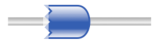
\includegraphics[height=6mm]{rep3}   & Yes   & lambdoid & SL2549 \\
    SLP281 & 2815382 - 2825915 & SL2633 & 2 X Phage\_CI\_repr (PF07022) &   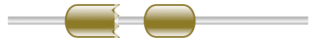
\includegraphics[height=6mm]{rep4}    & Yes   & degenerate P2-like & N/A \\
    Fels-2 SLP285 & 2855616 - 2888522 & SL2708 & Phage\_CI\_repr (PF07022) &   
\includegraphics[height=6mm]{rep5}    & Yes   & P2-like & SL2695 \\
    SLP289 & 2890073 - 2900377 & IsrK RNA (RF01394) & N/A   & N/A   & No    & P4-like & N/A \\
    SLP443 & 4437731 - 4459844 & N/A   & N/A   & N/A   & No    & remnant & SL4132 \\
    \bottomrule    
    \end{tabular}%
    \label{tab:stm_phage}%
\end{table}



{\it S.} Typhimurium and {\it S.} Typhi both contains 8 apparent large phage-derived genomic regions \parencite{Thomson2004, Kropinski2007}.  We were able to identify required repressors in all the intact lambdoid, P2-like, and P22-like prophage in both genomes, including Gifsy-1, Gifsy-2, and Fels-2/SopE (see tables \ref{tab:stm_phage} and \ref{tab:ty_phage}). With the exception of the SLP203 P22-like prophage in {\it S.} Typhimurium, all of these repressors lack the peptidase domain of the classical $\lambda$ repressor gene cI. This implies that the default anti-repression mechanism of Salmonella prophage may be more similar to a trans-acting mechanism recently discovered in Gifsy phage \parencite{Lemire2011} than to the $\lambda$ repressor's RecA-induced self-cleavage mechanism. We are also able to confirm that most phage remnants and fusions contained no active repressors, with the exception of the SLP281 degenerate P2-like prophage in {\it S.} Typhimurium. This degenerate prophage contains both intact replication and integration genes, but appears to lack tail and head proteins, suggesting it may depend on another phage for production of viral particles. Both genomes also encode P4-like satellite prophage, which rely on `helper' phage for lytic functions and utilize a complex antisense-RNA based regulation mechanism for decision pathways regarding cell fate \parencite{Briani2001} using structural homologs of the IsrK \parencite{Padalon-Brauch2008} and C4 ncRNAs \parencite{Forti2002}, known as seqA and CI RNA in the P4 literature, respectively. While the mechanism of P4 lysogenic maintenance is not known, the IsrK-like ncRNAs of two potentially active P4-like prophage in {\it S.} Typhi are required under TraDIS. This sequence element has previously been shown to be essential for the establishment of the P4 lysogenic state \parencite{Sabbattini1995}, and we predict based on our observations that it may be necessary for lysogenic maintenance as well. The fact that some lambdoid prophage in {\it S.} Typhimurium encode non-coding genes structurally similar to the IsrK-C4 immunity system of P4 raises the possibility that these systems may be acting as a defense mechanism of sorts, protecting the prophage from predatory satellite phage capable of co-opting its lytic genes.

% Table generated by Excel2LaTeX from sheet 'Sheet1'
%
\begin{table}
   \tiny
   \centering
   \noindent
    \caption[Phage elements in \textit{S.} Typhi]{\textbf{Phage elements in \emph{S.} Typhi.} Genomic coordinates determined from \textcite{Thomson2004} and manual inspection. Repressor domains and architecture were determined using the HMMER webserver \parencite{Finn2011} and Pfam \parencite{Punta2012}. Phage types were determined using repressor sequence similarity searches and information from \textcite{Thomson2004} and \textcite{Kropinski2007}. }
    \begin{tabular}{     m{0.5in}
    				m{0.4in}
				m{0.4in}
				m{0.6in}
				m{1.6in}
				m{0.4in}
				m{0.5in}
				m{0.5in}
				}
   
    \\
     \toprule
    \textbf{Element name} & \textbf{Genomic coordinates} & \textbf{Repressor} & \textbf{Repressor domain(s)} & \textbf{Repressor domain architecture} & \textbf{Predicted active?} & \textbf{Phage type} & \textbf{Required cargo} \\
    \midrule
    ST15  & 1408790 - 1441377 & N/A   & N/A   & N/A   & No    & Mu/P2 fusion & N/A \\
    Gifsy-2 & 1929572 - 1972330 & t1920 & HTH\_3 (PF01381) &    
\includegraphics[height=6mm]{rep6}   & Yes   & lambdoid & N/A \\
    ST2-27 & 2735054 - 2745321 & IsrK RNA (RF01394) & N/A   & N/A   & Yes   & P4-like & N/A \\
    ST27  & 2745477 - 2768221 & N/A   & N/A   & N/A   & No    & P2/iroA fusion & N/A \\
    ST35  & 3500854 - 3536047 & t3402 & Phage\_CI\_repr (PF07022) &   
\includegraphics[height=6mm]{rep7}    & Yes   & P2-like & t3415 \\
    SopE  & 4457346 - 4491316 & t4337 & Phage\_CI\_repr (PF07022) &   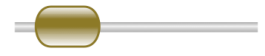
\includegraphics[height=6mm]{rep8}    & Yes   & P2-like & N/A \\
    N/A   & 4519423 - 4519501 & IsrK RNA (RF01394) & N/A   & N/A   & No    & remnant & N/A \\
    ST46  & 4666579 - 4677433 & IsrK RNA (RF01394) & N/A   & N/A   & Yes   & P4-like & N/A \\
    \bottomrule
    \end{tabular}%
    \label{tab:ty_phage}%
\end{table}



In addition to repressors, 4 prophage cargo genes in {\it S.} Typhimurium and one in {\it S.} Typhi are required (See tables \ref{tab:stm_phage}, \ref{tab:ty_phage}, \ref{tab:stm_uniq}, and \ref{tab:ty_uniq}). The {\it S.} Typhimurium prophage cargo genes encode a PhoPQ regulated protein, a protein predicted to be involved in natural transformation, an endodeoxyribonuclease, and a hypothetical protein. The {\it S.} Typhi prophage cargo gene encodes a protein containing the DNA-binding HIRAN\nomenclature[Z]{HIRAN}{HIP116, Rad5p N-terminal} domain \parencite{Iyer2006}, believed to be involved in the repair of damaged DNA. These warrant further investigation, as they are genes that have been recently acquired and become necessary for survival in rich media.

To compare differences between requirements for orthologous genes in both serovars, we calculated log-fold read ratios to eliminate genes which were classified differently in {\it S.} Typhi and {\it S.} Typhimurium but did not have significantly different read densities (see Methods.) Even after this correction, 36 {\it S.} Typhimurium genes had a significantly lower frequency of transposon insertion compared to the equivalent genes in {\it S.} Typhi (P $<$ 0.05), including four encoding hypothetical proteins (table \ref{stm_uniq}). This indicates that these gene products play a vital role in {\it S.} Typhimurium but not in {\it S.} Typhi when grown under laboratory conditions. 

% Table generated by Excel2LaTeX from sheet 'Sheet1'
%
\definecolor{Gray}{gray}{0.9}
\begingroup
\begin{landscape}
   \tiny
   \noindent
    \begin{longtable}{ r
    				r
				r
				r
				r
				l
				r
				r
				r
				c
				p{1.8in}}
    \caption[Genes uniquely required in {\it S.} Typhimurium]{\textbf{Genes uniquely required in {\it S.} Typhimurium.} Genes determined to be uniquely required in {\it S.} Typhimurium. SL, {\it S.} Typhimurium; Ty, {\it S.} Typhi; inserts refer to the number of unique insertion sites within a gene; reads refer to the number of sequence reads over all insertions sites within a gene. \textdagger, P-value (associated with log2 read ratio) < 0.05. \textdaggerdbl, {\it sseJ} is a pseudogene in S. Typhi. Shaded rows indicate genes shown to be H-NS repressed in \textcite{Navarre2006}}
    \\
       \toprule
   & \textbf{Ty inserts} & \textbf{Ty reads} & \textbf{SL inserts} & \textbf{SL reads} & \textbf{SL ID} & \textbf{SL gene length} & \textbf{Ty ID} & \textbf{Ty gene length} & \textbf{Name} & \textbf{Function} \\
    \midrule
\multirow{22}{*}{\begin{sideways}\textbf{No ortholog in {\it S.} Typhi}\end{sideways}}   & -     & -     & 18    & 123   & SL0742 & 1269  & -     & -     & -     & putative cation transporter \\
   &\cellcolor{Gray}-     &\cellcolor{Gray}-     &\cellcolor{Gray}9     &\cellcolor{Gray}80    &\cellcolor{Gray}SL0830 &\cellcolor{Gray}516   &\cellcolor{Gray}-     &\cellcolor{Gray}-     &\cellcolor{Gray}-     &\cellcolor{Gray}conserved hypothetical protein \\
   &\cellcolor{Gray}-     &\cellcolor{Gray}-     &\cellcolor{Gray}4     &\cellcolor{Gray}21    & \cellcolor{Gray}SL0831 &\cellcolor{Gray}855   &\cellcolor{Gray}-     &\cellcolor{Gray}-     &\cellcolor{Gray}-     & \cellcolor{Gray}putative electron transfer flavoprotein (beta subunit) \\
   & -     & -     & 0     & 0     & SL0950 & 323   & -     & -     & -     & predicted bacteriophage protein, potential phage repressor Gifsy-2 \\
   & -     & -     & 11    & 75    & SL1179 & 789   & -     & -     & envF  & lipoprotein \\
   & -     & -     & 3     & 18    & SL1480 & 249   & -     & -     & -     & antitoxin Phd\_YefM, type II toxin-antitoxin system \\
   & -     & -     & 4     & 32    & SL1527 & 264   & -     & -     & ydcX  & putative inner membrane protein \\
   &\cellcolor{Gray}-     &\cellcolor{Gray}-     &\cellcolor{Gray}1     &\cellcolor{Gray}3     &\cellcolor{Gray}SL1560 &\cellcolor{Gray}717   &\cellcolor{Gray}-     &\cellcolor{Gray}-     &\cellcolor{Gray}-     &\cellcolor{Gray}putative membrane protein \\
   & -     & -     & 7     & 50    & SL1601 & 859   & -     & -     & -     & putative transcriptional regulator (pseudogene) \\
   & -     & -     & 4     & 36    & SL1799 & 201   & -     & -     & -     & bacteriophage encoded pagK (phoPQ-activated protein) \\
   & -     & -     & 5     & 22    & SL1830A & 434   & -     & -     & -     & conserved hypothetical protein (pseudogene) \\
   & -     & -     & 3     & 27    & SL1967 & 677   & -     & -     & -     & predicted bacteriophage protein, potential phage repressor SLP203 \\
   & -     & -     & 1     & 15    & SL2045A & 63    & -     & -     & yoeI  & short ORF \\
   & -     & -     & 17    & 107   & SL2066 & 900   & -     & -     & rfbJ  & CDP-abequose synthase \\
   & -     & -     & 3     & 34    & SL2549 & 209   & -     & -     & -     & endodeoxyribonuclease \\
   & -     & -     & 4     & 149   & SL2593 & 449   & -     & -     & -     & putative DNA-binding protein, potential phage repressor Gifsy-1 SLP272 \\
   & -     & -     & 3     & 7     & SL2633 & 846   & -     & -     & -     & putative repressor protein, phage SLP281 \\
   & -     & -     & 2     & 21    & SL2695 & 978   & -     & -     & smf   & putative competence protein \\
   & -     & -     & 5     & 39    & SL4132 & 291   & -     & -     & -     & hypothetical protein \\
   & -     & -     & 5     & 45    & SL4354A & 303   & -     & -     & -     & conserved hypothetical protein \\
   \midrule
  \multirow{11}{*}{\begin{sideways}\parbox{2in}{\centering\textbf{Present in {\it S.} Typhi but required only in {\it S.} Typhimurium}\textsuperscript{\textdagger}}\end{sideways}} & 36    & 474   & 5     & 26    & SL0032 & 441   & t0033 & 306   & -     & putative transcriptional regulator \\
   & 71    & 349   & 11    & 48    & SL0623 & 642   & t2232 & 576   & lipB  & lipoate-protein ligase B \\
   & 151   & 3546  & 10    & 64    & SL0702 & 897   & t2156 & 894   & -     & putative glycosyl transferase \\
   & 194   & 3007  & 9     & 61    & SL0703 & 1134  & t2155 & 1134  & -     & galactosyltransferase \\
   & 231   & 3499  & 15    & 67    & SL0706 & 1779  & t2152 & 1780  & -     & putative glycosyltransferase, cell wall biogenesis \\
   & 84    & 1041  & 2     & 4     & SL0707 & 834   & t2151 & 834   & -     & putative glycosyltransferase, cell wall biogenesis \\
   & 49    & 367   & 14    & 70    & SL0722 & 1569  & t2136 & 1569  & cydA  & cytochrome d ubiquinol oxidase subunit I \\
   &\cellcolor{Gray}74    &\cellcolor{Gray}1613  &\cellcolor{Gray}5     &\cellcolor{Gray}22    &\cellcolor{Gray}SL1069 &\cellcolor{Gray}693   &\cellcolor{Gray}t1789 &\cellcolor{Gray}693   &\cellcolor{Gray}-     &\cellcolor{Gray}putative secreted protein \\
   & 20    & 199   & 1     & 1     & SL1203 & 150   & t1146 & 156   & -     & hypothetical protein \\
   & 20    & 290   & 1     & 5     & SL1264 & 315   & t1209 & 315   & -     & putative membrane protein \\
   &\cellcolor{Gray}84    &\cellcolor{Gray}384   &\cellcolor{Gray}6     &\cellcolor{Gray}26    &\cellcolor{Gray}SL1327 &\cellcolor{Gray}402   &\cellcolor{Gray}t1261 &\cellcolor{Gray}384   &\cellcolor{Gray}spiC  &\cellcolor{Gray}putative pathogenicity island 2 secreted effector protein \\
    \multirow{25}{*}{\begin{sideways}\parbox{3in}{\centering\textbf{Present in {\it S.} Typhi but required \\only in {\it S.} Typhimurium}}\end{sideways}}&\cellcolor{Gray}66    &\cellcolor{Gray}769   &\cellcolor{Gray}5     &\cellcolor{Gray}35    &\cellcolor{Gray}SL1331 &\cellcolor{Gray}270   &\cellcolor{Gray}t1265 &\cellcolor{Gray}327   &\cellcolor{Gray}sseA  & \cellcolor{Gray}T3SS chaperone \\
   &\cellcolor{Gray}36    &\cellcolor{Gray}307   &\cellcolor{Gray}2     &\cellcolor{Gray}5     &\cellcolor{Gray}SL1341 &\cellcolor{Gray}228   & \cellcolor{Gray}t1275 &\cellcolor{Gray}228   &\cellcolor{Gray}ssaH  &\cellcolor{Gray}putative pathogenicity island protein \\
   &\cellcolor{Gray}47    & \cellcolor{Gray}407   &\cellcolor{Gray}1     & \cellcolor{Gray}3     &\cellcolor{Gray}SL1342 &\cellcolor{Gray}249   &\cellcolor{Gray}t1276 &\cellcolor{Gray}249   &\cellcolor{Gray}ssaI  &\cellcolor{Gray}putative pathogenicity island protein \\
   &\cellcolor{Gray}144   &\cellcolor{Gray}3197  &\cellcolor{Gray}5     &\cellcolor{Gray}14    &\cellcolor{Gray}SL1343 &\cellcolor{Gray}750   &\cellcolor{Gray}t1277 &\cellcolor{Gray}750   &\cellcolor{Gray}ssaJ  &\cellcolor{Gray}putative pathogenicity island lipoprotein \\
   &\cellcolor{Gray}63    &\cellcolor{Gray}847   &\cellcolor{Gray}5     &\cellcolor{Gray}26    &\cellcolor{Gray}SL1354 &\cellcolor{Gray}267   &\cellcolor{Gray}t1288 &\cellcolor{Gray}267   &\cellcolor{Gray}ssaS  &\cellcolor{Gray}putative type III secretion protein \\
   &\cellcolor{Gray}73    &\cellcolor{Gray}762   &\cellcolor{Gray}4     &\cellcolor{Gray}44    &\cellcolor{Gray}SL1355 &\cellcolor{Gray}780   &\cellcolor{Gray}t1289 &\cellcolor{Gray}780   &\cellcolor{Gray}ssaT  &\cellcolor{Gray}putative type III secretion protein \\
   & 30    & 226   & 12    & 48    & SL1386 & 693   & t1322 & 693   & rnfE/ydgQ & Electron transport complex protein rnfE \\
   &\cellcolor{Gray}265   &\cellcolor{Gray}3337  &\cellcolor{Gray}29    &\cellcolor{Gray}165   &\cellcolor{Gray}SL1473 &\cellcolor{Gray}1557  &\cellcolor{Gray}t1463 &\cellcolor{Gray}1557  &\cellcolor{Gray}pqaA  &\cellcolor{Gray}PhoPQ-activated protein \\
   &\cellcolor{Gray}85    &\cellcolor{Gray}765   &\cellcolor{Gray}6     &\cellcolor{Gray}35    &\cellcolor{Gray}SL1532 &\cellcolor{Gray}951   &\cellcolor{Gray}t1511 &\cellcolor{Gray}951   &\cellcolor{Gray}sifB  &\cellcolor{Gray}putative virulence effector protein \\
   &\cellcolor{Gray}22    &\cellcolor{Gray}156   &\cellcolor{Gray}16    &\cellcolor{Gray}174   &\cellcolor{Gray}SL1561 &\cellcolor{Gray}1227  &\cellcolor{Gray}t1534\textsuperscript{\textdaggerdbl} &\cellcolor{Gray}141   &\cellcolor{Gray}sseJ  &\cellcolor{Gray}Salmonella translocated effector protein (SseJ) \\
   &\cellcolor{Gray}119   &\cellcolor{Gray}1639  &\cellcolor{Gray}10    &\cellcolor{Gray}44    &\cellcolor{Gray}SL1563 &\cellcolor{Gray}762   &\cellcolor{Gray}t1536 &\cellcolor{Gray}762   &\cellcolor{Gray}-     &\cellcolor{Gray}putative periplasmic amino acid-binding protein \\
   &\cellcolor{Gray}107   &\cellcolor{Gray}2440  &\cellcolor{Gray}5     &\cellcolor{Gray}44    &\cellcolor{Gray}SL1564 &\cellcolor{Gray}648   &\cellcolor{Gray}t1537 &\cellcolor{Gray}648   &\cellcolor{Gray}-     &\cellcolor{Gray}putative ABC amino acid transporter permease \\
   &\cellcolor{Gray}183   &\cellcolor{Gray}1646  &\cellcolor{Gray}20    &\cellcolor{Gray}118   &\cellcolor{Gray}SL1628 &\cellcolor{Gray}1355  &\cellcolor{Gray}t1612 &\cellcolor{Gray}1364  &\cellcolor{Gray}-     &\cellcolor{Gray}hypothetical protein \\
   &\cellcolor{Gray}23    &\cellcolor{Gray}177   &\cellcolor{Gray}1     &\cellcolor{Gray}5     &\cellcolor{Gray}SL1659 &\cellcolor{Gray}183   &\cellcolor{Gray}t1640 & \cellcolor{Gray}183   &\cellcolor{Gray}yciG  &\cellcolor{Gray}conserved hypothetical protein \\
   & 78    & 617   & 16    & 104   & SL1684 & 1014  & t1664 & 1014  & hnr   & putative regulatory protein \\
   &\cellcolor{Gray}37    &\cellcolor{Gray}277   &\cellcolor{Gray}4     &\cellcolor{Gray}25    &\cellcolor{Gray}SL1785 &\cellcolor{Gray}396   &\cellcolor{Gray}t1022 &\cellcolor{Gray}396   &\cellcolor{Gray}-     &\cellcolor{Gray}conserved hypothetical protein \\
   &\cellcolor{Gray}166   &\cellcolor{Gray}2823  &\cellcolor{Gray}9     &\cellcolor{Gray}27    &\cellcolor{Gray}SL1793 &\cellcolor{Gray}915   &\cellcolor{Gray}t1016 &\cellcolor{Gray}915   &\cellcolor{Gray}pagO  &\cellcolor{Gray}inner membrane protein \\
   &\cellcolor{Gray}28    &\cellcolor{Gray}311   &\cellcolor{Gray}3     &\cellcolor{Gray}22    &\cellcolor{Gray}SL1794 &\cellcolor{Gray}159   &\cellcolor{Gray}t1015 & \cellcolor{Gray}159   &\cellcolor{Gray}-     &\cellcolor{Gray}putative inner membrane protein \\
   & 23    & 155   & 1     & 4     & SL1823 & 972   & t0988 & 972   & msbB  & lipid A acyltransferase \\
   & 60    & 402   & 11    & 58    & SL2064 & 1002  & t0786 & 1002  & rfbV  & putative glycosyl transferase \\
   & 87    & 524   & 7     & 59    & SL2065 & 1293  & t0785 & 1299  & rfbX  & putative O-antigen transporter \\
   & 66    & 559   & 13    & 74    & SL2069 & 774   & t0780 & 774   & rfbF  & glucose-1-phosphate cytidylyltransferase \\
   & 41    & 204   & 5     & 14    & SL3828 & 1830  & t3658 & 1830  & glmS  & glucosamine-fructose-6-phosphate aminotransferase \\
   & 27    & 288   & 5     & 23    & SL4250 & 288   & t4220 & 288   & -     & putative GerE family regulatory protein \\
   & 148   & 2633  & 16    & 89    & SL4251 & 876   & t4221 & 876   & -     & araC family regulatory protein \\
    \bottomrule
    \label{tab:stm_uniq}%
    \end{longtable}%
\end{landscape}%
\endgroup



\begin{figure}[htp]
\begin{center}
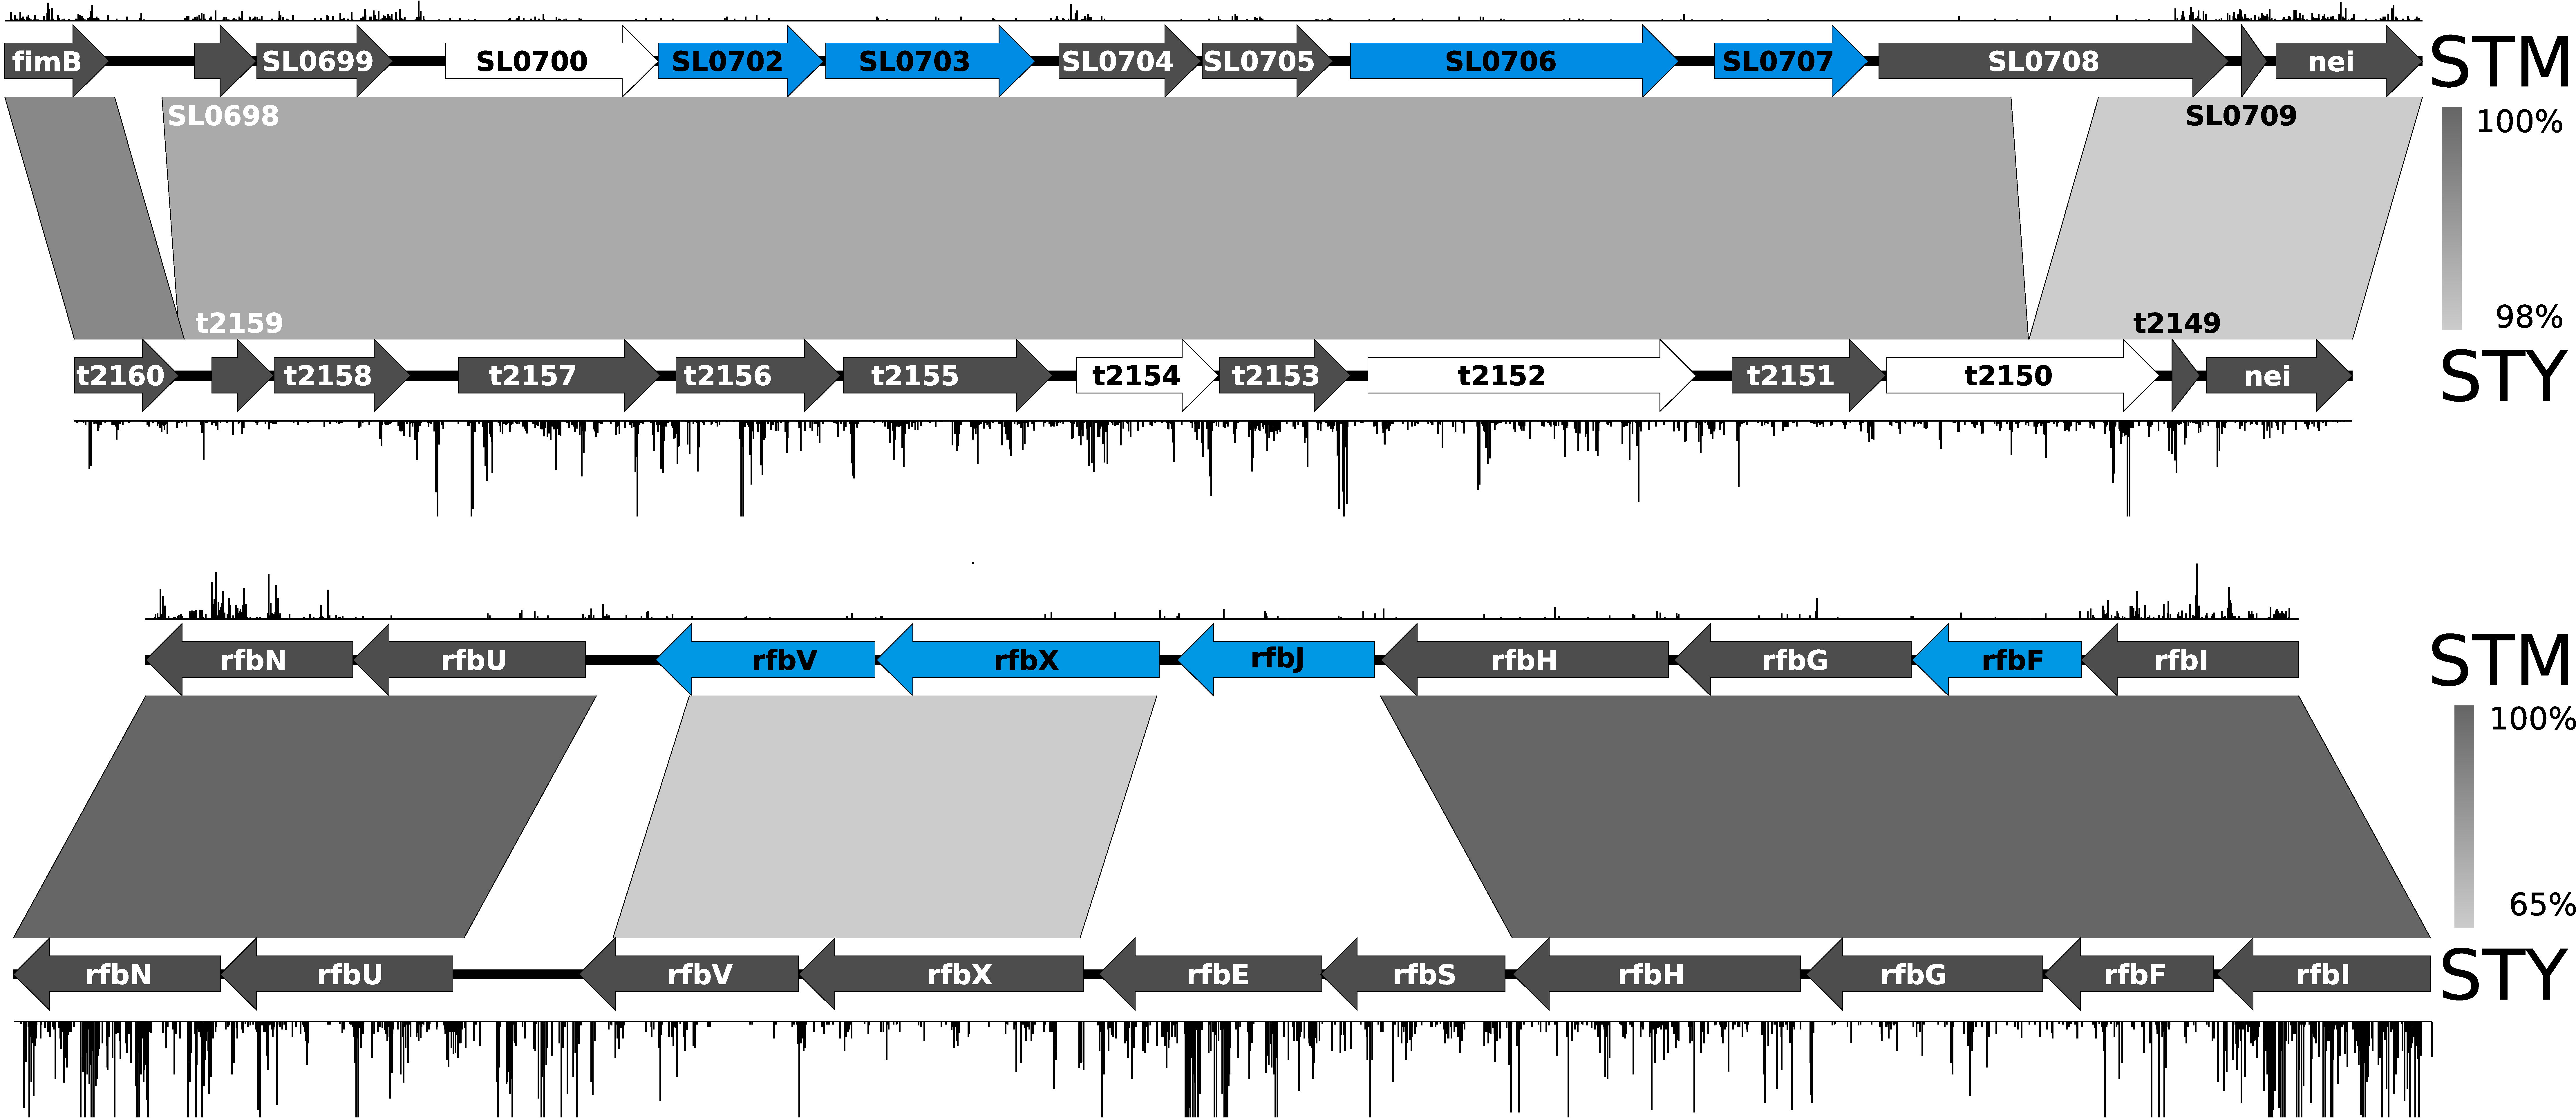
\includegraphics[width=14cm]{cell_surface}
\caption[Comparison of cell surface operon structure and requirements]{\textbf{Comparison of cell surface operon structure and requirements.} Diagram illustrating cell surface operons with different requirement patterns in {\it S.} Typhimurium and {\it S.} Typhi. The top figure is of an uncharacterized operon putatively involved in cell wall biogenesis, while the bottom figure shows a portion of the rfb operon involved in O-antigen biosynthesis. Plots along the top and bottom of each figure show insertions in {\it S.} Typhimurium and {\it S.} Typhi, respectively, with read depth on the y-axis with a maximum cut-off of 100 reads. Genes in blue are required in {\it S.} Typhimurium, genes in white are pseudogenes; others are in grey. Grey rectangles represent BLAST hits between orthologous genes, with percent nucleotide identity colored on the scale to the right of each figure.
} 
\label{fig:cell_surface}
\end{center}
\end{figure}

A major difference between the two serovars is in the requirement for genes involved in cell wall biosynthesis (see figure \ref{fig:cell_surface}). A set of four genes (SL0702, SL0703, SL0706, and SL0707) in an operonic structure putatively involved in cell wall biogenesis is required in {\it S.} Typhimurium but not in {\it S.} Typhi. The protein encoded by SL0706 is a pseudogene in {\it S.} Typhi (Ty2 unique ID: t2152) due to a 1bp deletion at codon 62 that causes a frameshift (Figure 4a). This operon contains an additional two pseudogenes in {\it S.} Typhi (t2154 and t2150), as well as a single different pseudogene (SL0700) in {\it S.} Typhimurium, indicating that this difference in gene requirements reflects the evolutionary adaptation of these serovars to their respective niches. Similarly, four genes ({\it rfbV}, {\it rfbX}, {\it rfbJ} and {\it rfbF}) within an O-antigen biosynthetic operon are required by {\it S.} Typhimurium but not {\it S.} Typhi. There appears to have been a shuffling of O-antigen biosynthetic genes since the divergence between the two serovars, and {\it rfbJ}, encoding a CDP-abequose\nomenclature[Z]{CDP}{Cytidine diphosphate glucose} synthase, has been lost from {\it S.} Typhi altogether. These broader requirements for cell wall-associated biosynthetic and transporter genes suggest that surface structure biogenesis is of greater importance in {\it S.} Typhimurium.

We also identified seven genes from the shared pathogenicity island SPI-2 that appear to contain few or no transposon insertions only in {\it S.} Typhimurium under laboratory conditions. These genes ({\it spiC}, {\it sseA}, and {\it ssaHIJT}) are thought to encode components of the SPI-2 type III secretion system apparatus (T3SS)\nomenclature[Z]{T3SS}{Type III secretion system} \parencite{Kuhle2004}. In addition, the effector genes {\it sseJ} and {\it sifB}, whose products are secreted through the SPI-2-encoded T3SS \parencite{Miao2000, Freeman2003}, also fell into the `required' category in {\it S.} Typhimurium alone. All of these genes display high A+T nucleotide sequence and have been previously shown (in {\it S.} Typhimurium) to be strongly bound by the nucleoid associated protein H-NS, encoded by {\it hns} \parencite{Lucchini2006, Navarre2006}. Therefore, rather than being `required', it is instead possible that access for the transposon was sufficiently restricted that very few insertions occurred at these sites. In further support of this hypothesis, a comparison of the binding pattern of H-NS detected in studies using {\it S.} Typhimurium LT2 with the TraDIS results from the SPI-2 locus indicated that high regions of H-NS enrichment correlated well with both the {\it ssa} genes described here and with {\it sseJ} (see figure \ref{fig:hns}). An earlier study also suggests that high-density DNA binding proteins can block Mu, Tn5, and Tn10 insertion \parencite{Manna2007}; however, a genome-wide study of the effects of H-NS binding on transposition would be necessary to confirm this effect.

\begin{figure}[htp]
\begin{center}
\includegraphics[width=14cm]{hns}
\caption[H-NS enrichment across the SPI-2 locus]{\textbf{H-NS enrichment across the SPI-2 locus.} Based on data from \textcite{Lucchini2006} where a 2 fold enrichment of H-NS-bound DNA over a total genomic DNA control in a ChIP-on-chip experiment was taken to indicate regions of H-NS binding in {\it S.} Typhimurium strain LT2. Assuming these binding patterns are similar in the {\it S.} Typhimurium strain tested in this study, H-NS binding may have affected transposon access to genes in the SPI-2 locus. 
} 
\label{fig:hns}
\end{center}
\end{figure}

% Table generated by Excel2LaTeX from sheet 'Sheet1'
%
\begin{table}
   \tiny
   \centering
   \noindent
    \caption[Candidate required genes affected by H-NS binding in {\it S.} Typhimurium]{\textbf{Candidate required genes affected by H-NS binding in {\it S.} Typhimurium.} Genes identified by comparison with data from \textcite{Navarre2006}. Fold change values report the results of a ChIP-on-chip experiment, and indicate genes strongly bound by H-NS. }
    \begin{tabular}{ c
    				c
				c
				r
				l
				}
   
    \\
     \toprule
    \textbf{Gene} & \textbf{SL ID} & \textbf{STM ID} & \textbf{Fold change} & \textbf{Function} \\
    \midrule
    -     & SL0830 & STM0854 & -16.2 & conserved hypothetical protein \\
    -     & SL0831 & STM0855 & -33.8 & putative putative electron transfer flavoprotein (beta subunit) \\
    -     & SL1069 & STM1131 & -13.5 & putative putative secreted protein \\
    spiC  & SL1327 & STM1393 & -19.1 & putative pathogenicity island 2 secreted effector protein \\
    sseA  & SL1331 & STM1397 & -46   & Type three secretion system chaperone \\
    ssaH  & SL1341 & STM1407 & -8.8  & Type three secretion system apparatus \\
    ssaI  & SL1342 & STM1408 & -32.4 & putative putative pathogenicity island protein \\
    ssaJ  & SL1343 & STM1409 & -53.7 & putative putative pathogenicity island lipoprotein \\
            ssaS & SL1354 & STM1420 & -15.5 & putative putative type III secretion protein \\
    ssaT  & SL1355 & STM1421 & -33.9 & putative putative type III secretion protein \\
    pqaA  & SL1473 & STM1544 & -5.5  & PhoPQ-activated protein \\
    sifB  & SL1532 & STM1602 & -66.8 & putative putative virulence effector protein \\
    -     & SL1560 & STM1630 & -9.8  & putative putative membrane protein \\
    sseJ  & SL1561 & STM1631 & -48.6 & salmonella translocated effector protein (SseJ) \\
    -     & SL1563 & STM1633 & -91.9 & putative putative periplasmic amino acid-binding protein \\
    -     & SL1564 & STM1634 & -22.5 & putative putative ABC amino acid transporter permease \\
    -     & SL1628 & STM1698 & -101.4 & hypothetical protein \\
    -     & SL1659 & STM1728 & -17.3 & cytochrome b561 (cytochrome b-561) \\
    -     & SL1785 & STM1856 & -12.1 & conserved hypothetical protein \\
    pagO  & SL1793 & STM1862 & -11.9 & inner membrane protein (PagO) \\
    -     & SL1794 & STM1864 & -22.9 & putative inner membrane protein \\
    \bottomrule
    \end{tabular}%
    \label{tab:hns}%
\end{table}



Indeed, the generation of null {\it S.} Typhimurium mutants in {\it sseJ} and {\it sifB}, as well as many others generated at the SPI-2 locus suggest that these genes are not truly a requirement for growth in this serovar \parencite{Freeman2003,Hensel1997,Hensel1998,Ohlson2005}. While this is a reminder that the interpretation of gene requirement needs to be made with care, the effect of H-NS upon transposon insertion is not genome-wide. If this were the case, there would be an under-representation of transposon mutants in high A+T regions (known for H-NS binding), which is not what we observed. In total, only 21 required genes fall into the `{\it hns}-repressed' category described in \textcite{Navarre2006}(see table \ref{tab:hns}); the remainder (almost 400) contained sufficient transposon insertions to conclude they were non-required. In addition, we noted that all SPI-1 genes that encode another T3SS and are of high A+T content were also found to be non-required. This phenomenon was not observed in {\it S.} Typhi, possibly because the strain used harbors the pHCM1 plasmid, which encodes the H-NS-like protein {\it sfh} and has been shown to affect H-NS binding \parencite{Doyle2007,Dillon2010}.

Twenty-two {\it S.} Typhi genes had a significantly lower frequency of transposon insertion compared to orthologs in {\it S.} Typhimurium (P $<$ 0.05), indicating that they are required only in {\it S.} Typhi for growth under laboratory conditions (table \ref{tab:ty_uniq}), including the {\it fepBDGC} operon. This indicates a requirement for ferric (Fe(III)\nomenclature{Fe(III)}{Ferric iron}) rather than ferrous (Fe(II)\nomenclature{Fe(II)}{Ferrous iron}) iron. This can be explained by the presence of Fe(III) in the bloodstream, where {\it S.} Typhi can be found during typhoid fever \parencite{Wain1998}. These genes function to recover the ferric chelator enterobactin from the periplasm, acting with a number of proteins known to aid the passage of this siderophore through the outer membrane \parencite{Rabsch1999}. It has long been noted that {\it aroA} mutants of {\it S.} Typhi, deficient in their ability to synthesize enterobactin, exhibit severe growth defects on complex media, while similar mutants of {\it S.} Typhimurium grow normally under the same conditions \parencite{Edwards1988}, though the mechanism has not been clear. Our results suggest that this difference in growth of {\it aroA} mutants is caused by a requirement for iron uptake through the {\it fep} system in {\it S.} Typhi. During host adaptation, {\it S.} Typhi has accumulated pseudogenes in many iron transport and response systems \parencite{McClelland2004}, presumably because they are not necessary for survival in the niche {\it S.} Typhi occupies in the human host, which may have led to this dependence on {\it fep} genes. In contrast, {\it S.} Typhimurium generally causes intestinal rather than systemic infection and is able to utilize a wider range of iron sources, including Fe(II), a soluble form of iron present under anaerobic conditions such as those found in the intestine \parencite{Tsolis1996}. 

% Table generated by Excel2LaTeX from sheet 'Sheet1'
%
\definecolor{Gray}{gray}{0.9}
\begingroup
\begin{landscape}
\begin{table}
   \tiny
   \noindent
    \caption[Genes uniquely required in {\it S.} Typhi]{\textbf{Genes uniquely required in {\it S.} Typhi.} Genes determined to be uniquely required in {\it S.} Typhi. SL, {\it S.} Typhimurium; Ty, {\it S.} Typhi; inserts refer to the number of unique insertion sites within a gene; reads refer to the number of sequence reads over all insertions sites within a gene.  \textdagger, P-value (associated with log2 read ratio) $<$ 0.05. *, the assignment of recA as a required gene has been described previously\parencite{Langridge2009a}, but briefly is believed to be due to the presence of the priC pseudogene in Typhi.}
        \begin{tabular}{ r
    				r
				r
				r
				r
				l
				r
				l
				r
				c
				p{1.8in}}
    \\
        \toprule
   & \textbf{SL inserts} & \textbf{SL reads} & \textbf{Ty inserts} & \textbf{Ty reads} & \textbf{Ty ID} & \textbf{Ty gene length} & \textbf{SL ID} & \textbf{SL gene length} & \textbf{Name} & \textbf{Function} \\
    \midrule
  \multirow{7}{*}{\begin{sideways}\parbox{1in}{\centering\textbf{No ortholog in {\it S.} Typhimurium}}\end{sideways}}& -     & -     & 1     & 5     & t1332 & 132   & -     & -     & malY  & pseudogene \\
  & -     & -     & 2     & 32    & t1920 & 405   & -     & -     & -     & possible repressor protein, prophage 10/Gifsy-2 \\
  & -     & -     & 2     & 12    & t3157 & 165   & -     & -     & -     & conserved hypothetical protein \\
  & -     & -     & 2     & 12    & t3166 & 228   & -     & -     & -     & spurious ORF annotation overlapping the RnaseP/M1 RNA \\
  & -     & -     & 6     & 196   & t3402 & 570   & -     & -     & cI    & repressor protein, cs 73 prophage \\
  & -     & -     & 4     & 58    & t3415 & 741   & -     & -     & -     & HIRAN-domain family gene, potential DNA repair \\
  & -     & -     & 1     & 6     & t4531 & 150   & -     & -     & -     & hypothetical secreted protein \\
    \midrule
    \multirow{22}{*}{\begin{sideways}\parbox{2.8in}{\centering\textbf{Present in {\it S.} Typhi but required only in {\it S.} Typhimurium}\textsuperscript{\textdagger}}\end{sideways}} &199   & 1792  & 18    & 59    & t0095 & 1287  & SL0093 & 1287  & surA  & survival protein SurA precursor \\
    &45    & 498   & 3     & 22    & t0123 & 459   & SL0119 & 459   & yabB/mraZ & conserved hypothetical protein \\
    &120   & 589   & 11    & 32    & t0203 & 1281  & SL0203 & 1281  & hemL  & glutamate-1-semialdehyde 2,1-aminomutase \\
    &123   & 982   & 2     & 25    & t0224 & 1353  & SL0224 & 1353  & yaeL/rseP & Zinc metallopeptidase \\
    &67    & 452   & 1     & 14    & t0270 & 576   & SL2604 & 576   & rpoE  & RNA polymerase sigma-E factor \\
    &140   & 760   & 0     & 0     & t0587 & 2286  & SL2246 & 2286  & nrdA  & ribonucleoside-diphosphate reductase 1 alpha chain \\
    &113   & 641   & 15    & 42    & t2140 & 2802  & SL0718 & 2802  & sucA  & 2-oxoglutarate dehydrogenase E1 component \\
    &116   & 753   & 13    & 36    & t2177 & 1641  & SL0680 & 1641  & pgm   & phosphoglucomutase \\
    &80    & 542   & 9     & 15    & t2276 & 1008  & SL0580 & 1008  & fepD  & ferric enterobactin transport protein FepD \\
    &93    & 591   & 2     & 2     & t2277 & 990   & SL0579 & 990   & fepG  & ferric enterobactin transport protein FepG \\
    &64    & 508   & 5     & 6     & t2278 & 795   & SL0578 & 795   & fepC  & ferric enterobactin transport ATP-binding protein FepC \\
    &201   & 1129  & 12    & 116   & t2410 & 2355  & SL0444 & 2355  & lon   & Lon protease \\
    &95    & 518   & 8     & 20    & t2730 & 1062  & SL2809 & 1062  & recA* & recA protein \\
    &135   & 719   & 16    & 39    & t2996 & 1992  & SL3052 & 1947  & tktA  & transketolase \\
    &76    & 358   & 3     & 9     & t3120 & 1434  & SL3173 & 1434  & rfaE  & ADP-heptose synthase \\
    &213   & 1976  & 6     & 50    & t3265 & 1071  & SL3321 & 1071  & degS  & serine protease \\
    &43    & 448   & 3     & 10    & t3326 & 606   & SL3925 & 606   & yigP  & conserved hypothetical protein \\
    &124   & 571   & 17    & 36    & t3384 & 2025  & SL3872 & 2025  & rep   & ATP-dependent DNA helicase \\
    &175   & 1208  & 6     & 21    & t3621 & 2787  & SL3947 & 2787  & polA  & DNA polymerase I \\
    &117   & 797   & 9     & 13    & t3808 & 1047  & SL3677 & 1047  & waaF  & ADP-heptose-LPS heptosyltransferase II \\
    &176   & 1628  & 14    & 59    & t4153 & 1080  & SL4183 & 1080  & alr   & alanine racemase \\
    &140   & 1127  & 10    & 38    & t4411 & 951   & SL4294 & 951   & miaA  & tRNA delta-2-isopentenylpyrophosphate transferase \\
    \bottomrule
   \end{tabular}
    \label{tab:ty_uniq}%
    \end{table}%
\end{landscape}%
\endgroup



\subsection{TraDIS provides resolution sufficient to evaluate ncRNA contributions to fitness}
Under a Poisson approximation to the transposon insertion process, a region of 41 (in {\it S.} Typhimurium) or 60 bases (in {\it S.} Typhi) has only a 1\% probability of not containing an insertion. NcRNAs tend to be considerably shorter than their protein-coding counterparts, but this gives us sufficient resolution to assay most of the non-coding complement of the Salmonella genome. As a proof of principle, we performed an analysis of the best-understood class of small ncRNAs, the tRNAs. Francis Crick hypothesized that a single tRNA could recognize more than one codon through wobble recognition \parencite{Crick1966}, where a non-canonical G-U base pair is formed between the first (wobble) position of the anticodon and the third nucleotide in the codon. As a result, some codons are covered by multiple tRNAs, while others are covered non-redundantly by a single tRNA. We expect that singleton wobble-capable tRNAs, that is wobble tRNAs which recognize a codon uniquely, will be required. In addition, we inferred the requirement for other tRNAs through the non-redundant coverage of their codons and used this to benchmark our ability to use TraDIS to reliably interrogate short genomic intervals.

The {\it S.} Typhi and {\it S.} Typhimurium genomes encode 78 and 85 (plus one pseudogene) tRNAs respectively with 40 anticodons, as identified by tRNAscan-SE \parencite{Lowe1997}. In {\it S.} Typhi, 10 out of 11 singleton wobble tRNAs are predicted to be required or ambiguous, compared to 16 tRNAs below the ambiguous LLR cut-off overall (significant enrichment at the 0.05 level, two-tailed Fisher�s exact test p-value: 6.4e-08.) Similarly in {\it S.} Typhimurium, 9 of 11 singleton wobble tRNAs are required or ambiguous compared to 15 required or ambiguous tRNAs overall, again showing a significant enrichment of required tRNAs in this subset (Fisher�s exact test p-value: 5.2e-07.)  The one singleton wobble tRNA which is consistently not required in both serovars is the tRNA-Pro(GGG), which occurs within a 4-member codon family. It has previously been shown in {\it S.} Typhimurium that tRNA-Pro(UGG) can read all four proline codons in vivo due to a cmo5U34 modification to the anticodon, obviating the need for a functional tRNA-Pro(GGG) \parencite{Nasvall2004} and making this tRNA non-required. The other non-required singleton wobble tRNA in {\it S.} Typhimurium, tRNA-Leu(GAG), is similarly a member of a 4-member codon family. We predict tRNA-Leu(TAG) may also be capable of recognizing all 4 leucine codons in this serovar; Such a leucine ``four-way wobble'' has been previously inferred in at least one other bacterial species \parencite{Osawa1992,Marck2002}.

Of the 6 required non-wobble tRNAs in each serovar, four are shared. These include two non-wobble singleton tRNAs covering codons uniquely, as well as a tRNA with the ATG anticodon which is post-transcriptionally modified by the required protein MesJ/TilS to recognize the isoleucine codon ATA \parencite{Marck2002}. An additional two required tRNAs in both serovars, one shared and one with a differing anticodon, contain Gln anticodons and are part of a polycistronic tRNA operon containing other required tRNAs. This operon is conserved in E. coli with the exception of an additional tRNA-Gln at the 3' end that has been lost in the Salmonella lineage. It is possible that transposon insertions early in the operon may interfere with processing of the polycistronic transcript in to mature tRNAs. Finally, we do not observe insertions in a tRNA-Met and a tRNA-Val in {\it S.} Typhi and {\it S.} Typhimurium, respectively.

Using this analysis of the tRNAs we estimate a worst-case PPV for these short molecules ($\sim$76 bases) at 81\%, in line with our previous estimates for conserved protein-coding genes, and a FPR of $<$4\%, higher than for protein-coding genes but still well within the typical tolerance of high-throughput experiments. This assumes that the ``required'' operonic tRNA-Glns and the serovar-specific tRNA-Met and tRNA-Val are all false positives; it is not clear that this is in fact the case.

Surveying the shared required ncRNA content of both serovars (see table \ref{tab:ncrna}), we find that the RNA components of the signal recognition particle (SRP)\nomenclature[Z]{SRP}{Signal recognition particle} and RNase P, two universally conserved ncRNAs, are required as expected. The SRP is an essential component of the cellular secretion machinery, while Rnase P is necessary for the maturation of tRNAs. We also find a number of required known and potential cis-regulatory molecules associated with genes required for growth under laboratory conditions in both serovars. The FMN\nomenclature[Z]{FMN}{Flavin mononucleotide} riboswitch controls {\it ribB}, a 3,4-dihydroxy-2-butanone 4-phosphate synthase involved in riboflavin biosynthesis, in response to flavin mononucleotide concentrations \parencite{Winkler2002}. Additionally, we are able to assign putative functions to a number of previously uncharacterized required non-coding transcripts through their 5' association with required genes. SroE, a 90 nucleotide molecule discovered in an early sRNA screen \parencite{Vogel2003}, is consistently located at the 5' end of the required {\it hisS} gene across its phylogenic distribution in the Enterobacteriaceae. Given this consistent association and the function of HisS as a histidyl-tRNA synthetase, we hypothesize that this region may act in a manner similar to a T-box leader, inducing or repressing expression in response to tRNA-His levels. The {\it thrU} leader sequence, recently discovered in a deep-sequencing screen of E. coli \parencite{Raghavan2011}, appears to regulate a polycistronic operon of required singleton wobble tRNAs. Three additional required cis-regulatory elements, t44, S15, and StyR-8, are associated with required ribosomal proteins, highlighting the central role ncRNA elements play in regulating fundamental cellular processes. 
\newpage

% Table generated by Excel2LaTeX from sheet 'Sheet1'
%
\definecolor{Gray}{gray}{0.9}
\begingroup
   \tiny
   \noindent
    \begin{longtable}{ l
    				p{0.3in}
				p{1.5in}
				c
				p{0.5in}
				p{0.5in}
				p{1in}
				}
    \caption[Candidate required ncRNAs]{\textbf{Candidate required ncRNAs greater than 60 nucleotides in length, excluding rRNA and tRNA.} Known and putative non-coding elements classified as required or ambiguous in this screen. Required ncRNAs have a log-likelihood ratio (LLR) between required and non-required models of < -2; see Methods. * \textdagger, ncRNAs which are amibiguous (LLR between -2 and 2) in S. Typhi(*) or in S. Typhimurium(\textdagger). Hfq-binding annotations are taken from \textcite{Chao2012}. The downstream protein-coding genes columns report annotated CDS or ribosomal RNA start sites within 100 bases of each candidate required non-coding element on either strand, and whether these downstream sequences are also classified as required.}
    \\
     \toprule
    \textbf{Name} & \textbf{Rfam accession} & \textbf{Function} & \textbf{Hfq-binding} & \textbf{Downstream protein-coding gene(s)} & \textbf{Downstream gene required} & \textbf{References} \\
    \midrule
    \multicolumn{7}{l}{\textbf{Required or ambiguous in both {\it S.} Typhi and {\it S.} Typhimurium}}\\
    SRP   & RF00169 & RNA component of the signal recognition particle &       &       &       & \textcite{Rosenblad2009} \\
    RNase P & RF00010 & RNA component of RNase P &       & ybaZ  & N     & \textcite{Frank1998} \\
    RFN   & RF00050 & FMN-sensing riboswitch controlling the ribB gene &       & ribB  & Y     & \textcite{Winkler2002} \\
    SroE  & RF00371 & Putative cis-regulatory element controlling the hisS gene &       & hisS  & Y     & \textcite{Vogel2003} \\
    ThrU Leader & NA    & Putative cis-regulatory element controlling the ThrU tRNA operon &       &       &       & \textcite{Raghavan2011} \\
    t44   & RF00127 & Cis-regulatory element controlling the ribosomal rpsB gene &       & rpsB  & Y     & \textcite{Tjaden2002,Aseev2008,Meyer2009} \\
    S15\textsuperscript{\textdagger}  & RF00114 & Translational regulator of the ribosomal S15 protein &       & rpsO  & Y     & \textcite{Benard1996} \\
    StyR-8 & NA    & Putative cis-regulatory element controlling the ribosomal rpmB gene &       & rpmB  & Y     & \textcite{Chinni2010} \\
    MicA  & RF00078 & sRNA involved in cellular response to extracytoplasmic stress & Y     & luxS  & N     & \textcite{Vogel2009} \\
    DsrA\textsuperscript{\textdagger} & RF00014 & sRNA regulator of H-NS & Y     & mngB  & N     & \textcite{Lease1998} \\
    STnc10 & NA    & Putative sRNA &       & nhaA  & N     & \textcite{Sittka2008} \\
    STnc60\textsuperscript{\textdagger} & NA    & Putative sRNA &       &       &       & \textcite{Sittka2008} \\
    STnc840 & NA    & Verified sRNA derived from 3' UTR of the flgL gene & Y     &       &       & \textcite{Chao2012} \\
    IS0420*\textsuperscript{\textdagger} & NA    & Putative ncRNA &       & rmf   & N     & \textcite{Raghavan2011,Chen2002} \\
    RGO0\textsuperscript{\textdagger} & NA    & Putative sRNA identified in E. coli &       &       &       & \textcite{Raghavan2011} \\
     \multicolumn{7}{l}{\textbf{Required or ambiguous in {\it S.} Typhimurium only}}\\
    rne5  & RF00040 & RNase E autoregulatory 5' element  &       & rne   & Y     & \textcite{Diwa2000} \\
    RydC  & RF00505 & sRNA regulator of the yejABEF ABC transporter & Y     &       &       & \textcite{Antal2005} \\
    RydB  & RF00118 & Putative ncRNA &       &       &       & \textcite{Wassarman2001} \\
    STnc510 & NA    & Putative sRNA &       & pagD/pagC & Y/N   & \textcite{Sittka2008} \\
    STnc460\textsuperscript{\textdagger} & NA    & Putative sRNA &       &       &       & \textcite{Sittka2008} \\
    STnc170 & NA    & Putative sRNA &       & SL1458 & N     & \textcite{Sittka2008} \\
    STnc130 & NA    & Putative sRNA &       & dmsA  & N     & \textcite{Sittka2008} \\
    RseX  & RF01401 & sRNA regulator of OmpA and OmpC & Y     &       &       & \textcite{Douchin2006} \\
    IsrJ  & RF01393 & sRNA regulator of SPI-1 effector protein secretion &       &       &       &  \textcite{Sittka2008, Padalon-Brauch2008} \\
    IsrI  & RF01392 & Island-encoded Hfq-binding sRNA & Y     & SL1028 & Y     &  \textcite{Sittka2008, Padalon-Brauch2008, Chao2012} \\
     \multicolumn{7}{l}{\textbf{Required or ambiguous in {\it S.} Typhi only}}\\
    RybB  & RF00110 & sRNA involved in cellular response to extracytoplasmic stress & Y     &       &       &  \textcite{Vogel2009} \\
    tk5*  & NA    & Putative ncRNA &       &       &       & \textcite{Raghavan2011,Rivas2001} \\
    STnc750 & NA    & Verified sRNA & Y     & SpeB  & N     & \textcite{Kroger2012, Chao2012} \\
    StyR-44* & RF01830 & Putative multicopy (2/6 copies required in S. Typhi) ncRNA associated with ribosomal RNA operon &       & 23S rRNA & N     &  \textcite{Chinni2010} \\
    tp2   & NA    & Putative ncRNA &       & aceE  & N     &  \textcite{Raghavan2011,Rivas2001} \\
    RdlD  & RF01813 & RdlD RNA anti-toxin, 1/2 copies required in S. Typhi &       &       &       & \textcite{Kawano2002} \\
    STnc120* & NA    & Putative sRNA &       &       &       & \textcite{Sittka2008} \\
    tp28* & NA    & Putative ncRNA &       & fur   & N     &  \textcite{Raghavan2011,Rivas2001} \\
    Phe Leader* & RF01859 & Phenylalanine peptide leader sequence associated with the required PheST operon &       & PheS  & Y     & \textcite{Zurawski1978} \\
    RimP Leader & RF01770 & Putative cis-regulator of the rimP-nusA-infB operon &       & rimP  & Y     & \textcite{Naville2010} \\
    GlmY  & RF00128 & Trans-acting regulator of the GlmS gene &       &       &       & \textcite{Urban2008} \\
    \bottomrule
    \label{tab:ncrna}%
    \end{longtable}%
\endgroup



\subsection{sRNAs required for competitive growth}

Inferring functions for potential trans-acting ncRNA molecules, such as anti-sense binding small RNAs (sRNAs), from requirement patterns alone is more difficult than for cis-acting elements, as we cannot rely on adjacent genes to provide any information.  It is also important to keep in mind that TraDIS assays requirements after a brief competition within a large library of mutants on permissive media. This may be particularly important when surveying the bacterial sRNAs, which are known to participate in responses to stress \parencite{Vogel2009a}.  

\begin{figure}[htp]
\begin{center}
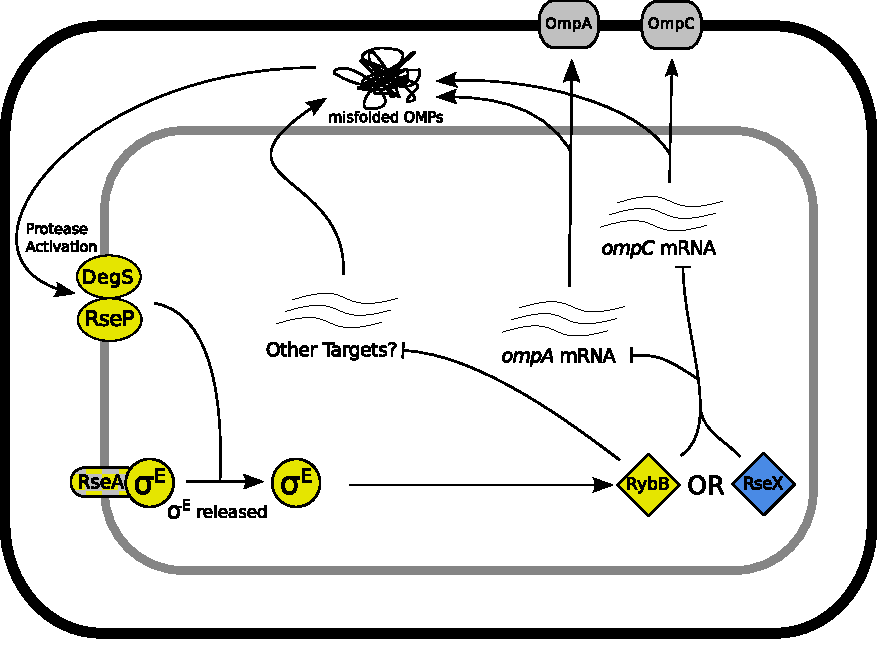
\includegraphics[width=14cm]{sRNAs}
\caption[Proposed differences in sRNA utilization]{\textbf{Proposed differences in sRNA utilization.} Diagram illustrating inferred required sRNA regulatory networks under TraDIS. Molecules required in {\it S.} Typhi are highlighted in yellow and in {\it S.} Typhimurium are highlighted in blue. RseA, in yellow/grey check, is ambiguous in {\it S.} Typhi. Non-required molecules are in grey. Diamonds indicate sRNAs, circles regulatory proteins, ovals proteases, oblong shapes are membrane-anchored proteins, and rounded squares are outer membrane porins.
} 
\label{fig:sRNAs}
\end{center}
\end{figure}

This is demonstrated by two sRNAs involved in the $\sigma^E$-mediated extracytoplamic\nomenclature[G]{$\sigma^E$}{$\sigma^{24}$, extracytoplasmic stress sigma factor} stress response, RybB and RseX, both of which can be successfully knocked out in {\it S.} Typhimurium (83). In {\it S.} Typhi, {\it rpoE} is required, as it also is in {\it E. coli} \parencite{Baba2006, DeLasPenas1997}. However, in {\it S.} Typhimurium, {\it rpoE} tolerates a heavy insertion load, implying that $\sigma^E$ mutants are not disadvantaged in competitive growth. In {\it S.} Typhimurium, the sRNA RseX is required. Overexpression of RseX has previously been shown to compensate for $\sigma^E$ essentiality in E. coli by leading to the degradation of {\it ompA} and {\it ompC} transcripts (85). This suggests that RseX may also be short-circuiting the $\sigma^E$ stress response network in {\it S.} Typhimurium (figure \ref{fig:sRNAs}). To our knowledge, this is the first evidence of a native (i.e. not experimentally induced) activity of RseX. 

{\it S.} Typhi on the other hand requires $\sigma^E$ along with its activating proteases RseP and DegS and anchoring protein RseA, as well as the $\sigma^E$-dependent sRNA RybB, which also regulates OmpA and OmpC in {\it S.} Typhimurium, along with a host of other OMPs\nomenclature[Z]{OMP}{Outer membrane protein} \parencite{Papenfort2006}. It is unclear why the $\sigma^E$ response is required in {\it S.} Typhi but not {\it S.} Typhimurium, though it may partially be due to the major differences in the cell wall and outer membrane between the two serovars. In addition, there are significant differences in the OMP content of the {\it S.} Typhi and {\it S.} Typhimurium membranes that may be driving alternative mechanisms for coping with membrane stress. For instance, {\it S.} Typhi completely lacks OmpD, a major component of the {\it S.} Typhimurium outer membrane \parencite{Santiviago2003} and a known target of RybB \parencite{Vogel2009a}. 

Two additional sRNAs involved in stress response are also required by both {\it S.} Typhi and {\it S.} Typhimurium. The first, MicA, is known to regulate {\it ompA} and the {\it lamB} porin-coding gene in {\it S.} Typhimurium \parencite{Bossi2007}, contributing to the extracytoplasmic stress response. The second, DsrA, has been shown to negatively regulate the nucleoid-forming protein H-NS and enhance translation of the stationary-phase alternative sigma factor $\sigma^S$\nomenclature[G]{$\sigma^S$}{$\sigma^{38}$, starvation/stationary phase sigma factor} in {\it E. coli} \parencite{Lease1998}, though its regulation of $\sigma^S$ does not appear to be conserved in {\it S.} Typhimurium \parencite{Jones2006}. Both have been previously deleted in {\it S.} Typhimurium, and so are not essential. H-NS knockouts have previously been shown to have severe growth defects in {\it S.} Typhimurium that can be rescued by compensatory mutations in either the {\it phoPQ} two-component system or {\it rpoS}, implying that the lack of H-NS is allowing normally silenced detrimental regions to be transcribed \parencite{Navarre2006}. As MicA has recently been shown to negatively regulate {\it phoPQ} expression in E. coli \parencite{Coornaert2010}, it is tempting to speculate that MicA may be moderating the effects of DsrA-induced H-NS repression; however, it is currently unclear whether sRNA regulons are sufficiently conserved between {\it E. coli} and {\it S.} enterica to justify this hypothesis.

\section{Conclusions}

The extremely high resolution of TraDIS has allowed us to assay gene requirements in two very closely related {\it Salmonellae} with different host ranges. We found, under laboratory conditions, that 58 genes present in both serovars were required in only one, suggesting that identical gene products do not necessarily have the same phenotypic effects in the two different serovar backgrounds. Many of these genes occur in genomic regions or metabolic systems which contain pseudogenes and/or have undergone reorganization since the divergence of {\it S.} Typhi and {\it S.} Typhimurium, demonstrating the complementarity of TraDIS and phylogenetic analysis. These changes may in part explain differences observed in the pathogenicity and host specificity of these two serovars. In particular, {\it S.} Typhimurium showed a requirement for cell surface structure biosynthesis genes; this may be partially explained by the fact that {\it S.} Typhi expresses the Vi-antigen which masks the cell surface, though these genes are not required for survival in our assay. {\it S.} Typhi on the other hand has a requirement for iron uptake through the {\it fep} system, which enables ferric enterobactin transport. This dependence on enterobactin suggests that {\it S.} Typhi is highly adapted to the iron-scarce environments it encounters during systemic infections. Furthermore, this appears to represent a single point of failure in the {\it S.} Typhi iron utilization pathways, and may present an attractive target for narrow-spectrum antibiotics. 

Of the approximately 4500 protein coding genes present in each serovar, only about 350 were sufficiently depleted in transposon insertions to be classified as required for growth in rich media. This means that over 92\% of the coding genome has sufficient insertion density to be queried in future assays. Dense transposon mutagenesis libraries have been used to assay gene requirements under conditions relevant for infection, including {\it S.} Typhi survival in bile \parencite{Langridge2009a}, {\it Mycobacterium tuberculosis} catabolism of cholesterol \parencite{Griffin2011}, drug resistance in {\it Pseudomonas aeruginosa} \parencite{Gallagher2011}, and {\it Haemophilus influenzae} survival in the lung \parencite{Gawronski2009}. We expect that parallel experiments querying gene requirements under the same conditions in both serovars examined in this study will yield further insights in to the differences in the infective process between Typhi and Typhimurium, and ultimately the pathways that underlie host-adaptation.

Both serovars possess substantial complements of horizontally-acquired DNA. We have been able to use TraDIS to assay these recently acquired sequences. In particular, we�ve been able to identify, on a chromosome wide scale, active prophage through the requirement for their repressors. The P4 phage utilizes an RNA-based system to make decisions regarding cell fate, and structurally similar systems are used by P1, P7, and N15 phage \parencite{Citron1990,Ravin1999}. C4-like transcripts have been regarded as the primary repressor of lytic functions, though the IsrK-like sequence is known to be essential to the establishment of lysogeny in P4 and is transcribed in at least two phage types \parencite{Sabbattini1995, Ravin1999}. Our observations in {\it S.} Typhi suggest an important role for the IsrK-like sequence in maintenance of the lysogenic state in P4-like phage, though the mechanism remains unclear.

Recent advances in high-throughput sequencing have greatly enhanced our ability to detect novel transcripts, such as ncRNAs and short open reading frames (sORFs). In fact, our ability to identify these transcripts now far out-strips our ability to experimentally characterize these sequences. There have been previous efforts at high-throughput characterization of bacterial sRNAs and sORFs in enteric bacteria; however, these have relied on labor-intensive directed knockout libraries \parencite{Santiviago2009, Hobbs2010}. Here we have demonstrated that TraDIS has sufficient resolution to reliably query genomic regions as short as 60 bases, in agreement with a recent high-throughput transposon mutagenesis study in the alphaproteobacteria {\it Caulobacter crescentus} \parencite{Christen2011}. Our method has the major advantage that library construction does not rely upon genome annotation, and newly discovered elements can be surveyed with no further laboratory work. 

We have been able to assign putative functions to a number of ncRNAs using TraDIS though consideration of their genomic and experimental context. In addition, ncRNA characterization generally is done in model organisms like {\it E. coli} or {\it S.} Typhimurium, and it is unclear how stable ncRNA regulatory networks are over evolutionary time. By assaying two serovars of {\it Salmonella} with the same method under the same conditions, we have seen hints that there may be differences in sRNA regulatory networks between {\it S.} Typhi and {\it S.} Typhimurium. In particular, we have found that under the same experimental conditions, {\it S.} Typhi appears to rely on the $\sigma^{E}$ stress response pathway while {\it S.} Typhimurium does not; it is tempting to speculate that this difference in stress response is mediated by the observed difference in requirement for two sRNAs, RybB and RseX. We believe that this combination of high-throughput transposon mutagenesis with a careful consideration of the systems context of individual genes provides a powerful tool for the generation of functional hypotheses. We anticipate that the construction of TraDIS libraries in additional organisms, as well as the passing of these libraries through relevant experimental conditions, will provide further insights into the function of bacterial ncRNAs in addition to the protein-coding gene complement. 

%% \pagebreak[4]
% \hspace*{1cm}
% \pagebreak[4]
% \hspace*{1cm}
% \pagebreak[4]
%\usepackage[round,colon,authoryear]{natbib}

\chapter{A pipeline for the analysis of TraDIS experiments, with an application to {\it Salmonella} macrophage invasion}
\label{sec:chapterPingpong}
\ifpdf
    \graphicspath{{Chapter3/Chapter3Figs/EPS/}{Chapter3/Chapter3Figs/}}
\fi

\textit{Section 3.3 describes a collaborative study with Gemma C. Langridge (Pathogen Genomics, Wellcome Trust Sanger Institute). Gemma performed all laboratory experiments described in this chapter.}

\section{Introduction}

In the previous chapter, I described the results of a study predicting and comparing the genes required for robust growth of two \textit{Salmonella} serovars in standard laboratory media. While this revealed interesting aspects of \textit{Salmonella} biology, linking these findings to \textit{Salmonella}'s infective niche in the human host is difficult. However, transposon-insertion sequencing can be used to interrogate infective conditions directly (reviewed previously in section 1.5): by comparing libraries passed through a condition of interest to control libraries, we can determine the genomic regions involved in survival in that condition. In this chapter, I describe a pipeline for the analysis of such experiments, illustrated with an experiment assaying genes required for \textit{S.} Typhi and Typhimurium invasion of (or uptake into) human macrophage.

\subsection{\textit{Salmonella} interactions with macrophage}

As previously described in section 2.1, the ability to invade and survive in host cells was a major factor in the early evolution of \textit{S. enterica} subspecies \textit{enterica}. This appears to have been largely driven by the acquisition of two horizontally-acquired pathogenicity islands, SPI-1 and -2. Due to the availability of a mouse model \parencite{Santos2001}, most of what is known about \textit{Salmonella} interactions with host cells is derived from studies of \textit{S.} Typhimurium infection. 

\textit{S.} Typhimurium infections of either epithelial or phagocytic cells appear to follow broadly similar paths (\textcite{Figueira2012}, see also figure \ref{fig:SCV}). On encountering a suitable host cell, the bacterium adheres, likely using an array of fimbrial adhesins \parencite{Baumler1996a, Velden1998}. The SPI-1 T3SS is induced, and  

\begin{figure}[htp]
\begin{center}
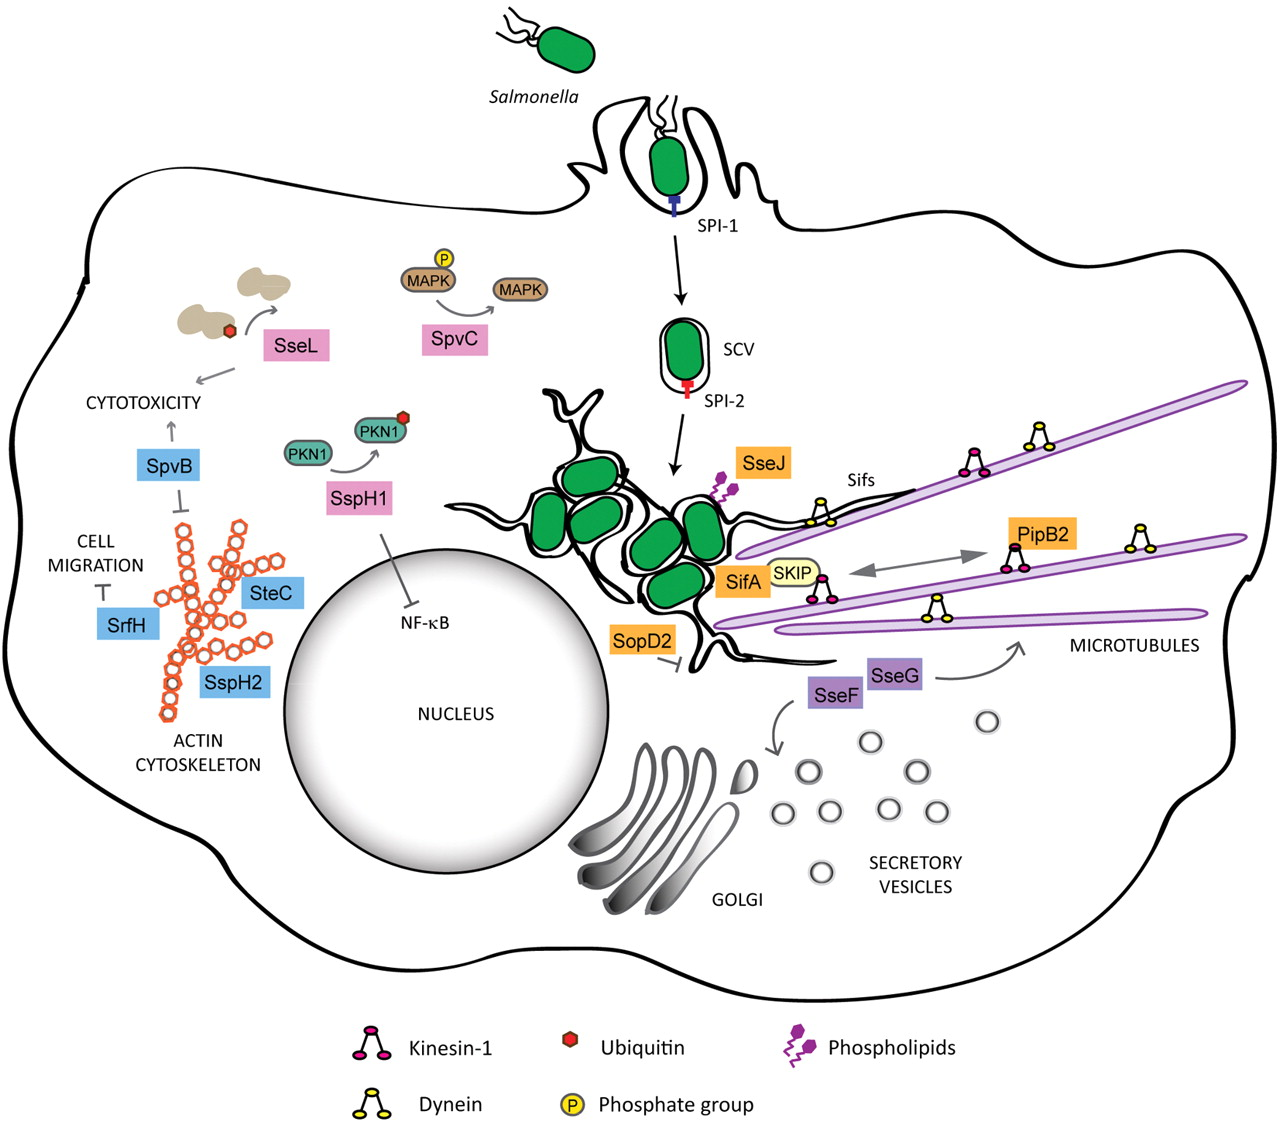
\includegraphics[width=14cm]{SCV.jpg}
\caption[Biogenesis of the \textit{Samonella} containing vacuole]{\textbf{Biogenesis of the \textit{Samonella} containing vacuole (SCV).} \textit{Salmonella} adheres to the outer membrane of host cells, and uses SPI-1 and its associated effectors to induce membrane ruffling and entry into the SCV. The SPI-2 T3SS functions mainly in maintenance of the SCV, through the action of the effectors SifA, SopD2, SseJ and PipB2 (orange boxes), and its localization near the Golgi of host cells, mediated by SseF and SseG (purple boxes). Other effectors are involved in modulation of host immune signalling (SpvC, SspH1 and SseL; pink boxes) or target the host cytoskeleton (SteC, SpvB, SspH2 and SrfH; blue boxes). Reproduced from \textcite{Figueira2012} under a Creative Commons Attribution License (CCAL). 
} 
\label{fig:SCV}
\end{center}
\end{figure}

\section{Methods}

Determining conditional gene fitness presents a somewhat different problem to that addressed in the previous chapter, predicting and comparing ``essential'' genes under the conditions of library creation. In predicting gene essentiality, we had a single time point representing the initial growth of the library on rich media, while in identifying conditional gene fitness (measured as the relative expansion or contraction of mutant populations) we are always comparing changes in mutant fitness with respect to fitness in a baseline condition. In some ways, this makes the problem of identifying genes with strong fitness effects easier: as we are primarily interested in the ratio of various insertion mutants present between the two conditions, effects that may confound the prediction of simple gene essentiality are effectively ``zeroed out''. More explicitly, whether low insertion density in the library occurs due to chance, nucleotide composition bias, or the exclusionary effects of high-density DNA-binding proteins (described in section 2.3.3) does not matter -- these regions can simply be identified as not producing sufficient reads over insertion-sites to be assayed and removed from the analysis.

In many ways, the problem of investigating the statistical and biological significance of ratios of reads over insertion sites resembles established analyses developed for differential RNA-seq analysis. In this section I describe the

\subsection{Mapping insertion sites}

\subsection{Defining genomic features}

\subsection{Quality control}

\subsection{Inter-library normalization}

\subsection{Identifying fitness effects}

\subsection{Functional analysis of gene sets that affect fitness}

\section{Application: \textit{Salmonella enterica} macrophage invasion}

\subsection{Background: the {\it Salmonella} containing vacuole}

\subsection{Experimental methods}

\textit{All experiments were performed by Gemma Langridge. They are described here briefly for completeness; in-depth descriptions of the experiments are available in \parencite{Langridge2010}}


\subsection{Results}

\subsection{Other applications}
%\include{Conclusions/conclusions}



\backmatter % book mode only
\fancyhead[LO,RE]{\textit{Published Works}}

% Thesis Published Work ---------------------------------------------------
\chapter{Publications}

Publications arising in the course of this thesis:

\itemize

\item{Okoro C.K., Barquist L., Kingsley R.A., Connor T.R., Harris S.R., Arends M., Stevens M., Parry C.M., Al-Mashhadani M.N., Kariuki S., Msefula C.L., Gordon M.A., de Pinna E., Wain J., Heyderman R.S., Obaro S., Alonso P.L., Mandomando I., MacLennan C.A., Tapia M.D., Levine M.M., Tennant S.M., Parkhill J., Dougan G.  \textbf{Signatures of adaptation in human invasive {\it S.} Typhimurium populations.} Manuscript in preparation, 2013.} 

\item{Pettit L.J., Browne H.P., Yu L., Smits W.K., Fagan R.P., Barquist L., Martin M.J., Goulding D., Duncan S.H., Flint H.J., Dougan G., Choudhary J.S., Lawley T.D. \textbf{\textit{Clostridium difficile} Spo0A coordinates sproulation, virulence and metabolism.} Manuscript in preparation, 2013.}

\item{Kingsley R.A., Whitehead S., Connor T., Barquist L., Sait L., Holt K., Sivaraman K., Wileman T., Goulding D., Clare S., Hale C., Seshasayee A., Harris S., Gardner P., Rabsch W., Wigley P., Humphrey T., Parkhill J., Dougan G. \textbf{Genome and transcriptome adaptation accompanied emergence of the DT2 host-adapted \textit{Salmonella} Typhimurium pathovar.} Manuscript under review, 2013.}

\newpage

\item{Reuter S., Connor T.R., Barquist L., Walker D., Feltwell T., Harris S.R., Fookes M., Hall M.E., Fuchs T.M., Corander J., Dufour M., Ringwood T., Savin C., Bouchier C., Martin L., Miettinen M., Shubin M., Laukkanen-Ninios R., Sihvonen L.M., Siitonen A., Skurnik M., Falc\~{a}o J.P., Fukushima H., Scholz H.C., Prentice M., Wren B.W., Parkhill J., Carniel E., Achtman M., McNally A., Thomson N.R. \textbf{Parallel independent evolution of pathogenicity within the genus \textit{Yersinia}.} Manuscript under review, 2013.}

\item{Croucher N.J., Mitchell A.M., Gould K.A., Inverarity D., Barquist L., Feltwell T., Fookes M.C., Harris S.R., Dordel J., Salter S.J., Browall S., Zemlickova H., Parkhill J., Normark S., Henriques-Normark B., Hinds J., Mitchell T.J., Bentley S.D. \textbf{Within-patient diversification and genomic stasis within a pneumococcal lineage.} Manuscript under review, 2013.} 

\item{Barquist L., Burge S.W., Gardner P.P. \textbf{Building non-coding RNA families.} \textit{Methods in Molecular Biology}, in press.} 

\item{Hoeppner M.P., Barquist L., Gardner P.P. \textbf{An introduction to RNA databases.} \textit{Methods in Molecular Biology}, in press.} 

\item{Martin M.J., Clare S., Goulding D., Faulds-Pain A., Barquist L., Browne H., Pettit L., Dougan G., Lawley T.D.,  Wren B.W. \textbf{The \textit{agr} locus regulates virulence and colonization genes in \textit{Clostridium difficile} 027.} \textit{Journal of Bacteriology}, 2013. }

\item{Barquist L., Boinett C.J., Cain A.K..  \textbf{Approaches to querying bacterial genomes with transposon-insertion sequencing.} \textit{RNA Biology}, 10(7), 2013.}

\item{Barquist L., Langridge G.C., Turner D.J., Phan M.D., Turner A.K., Bateman A., Parkhill J., Wain J., Gardner P.P. \textbf{A comparison of dense transposon insertion libraries in the \textit{Salmonella} serovars Typhi and Typhimurium.} \textit{Nucleic Acids Research}, 41(8):4549-4564, 2013.} 

\item{Burge S.W., Daub J., Eberhardt R., Tate J., Barquist L., Nawrocki E.P., Eddy S.R., Gardner P.P., Bateman A. \textbf{Rfam 11.0: 10 years of RNA families.} \textit{Nucleic Acids Research}. 41(D1):D226-D232, 2013}

\item{Croucher N.J., Harris S.R., Barquist L., Parkhill J., Bentley S.D. \textbf{A high-resolution view of genome-wide pneumococcal transformation.} \textit{PLoS Pathogens}, 8(6), 2012}

\item{Westesson O., Barquist L., Holmes I. \textbf{HandAlign: Bayesian multiple sequence alignment, phylogeny, and ancestral reconstruction.} \textit{Bioinformatics}, 28(8):1170-1171, 2012}

\item{Gardner P.P., Barquist L., Bateman A., Nawrocki E.P., Weinberg Z. \textbf{RNIE: genome-wide prediction of bacterial intrinsic terminators.} \textit{Nucleic Acids Research}, 39(14):5845-5852, 2011}



 
 % ----------------------------------------------------------------------

%%% Local Variables: 
%%% mode: latex
%%% TeX-master: "../thesis"
%%% End: 

\fancyhead[LO,RE]{\textit{Appendix}}

%\appendix
%\include{Appendix1/appendix1}
\clearpage
\fancyhead[LO,RE]{\textit{References}}
\addcontentsline{toc}{chapter}{References}
\renewcommand{\bibname}{References} % changes default name Bibliography to References
\singlespace
\printbibliography
\end{document}
